% Lines starting with a percent sign (%) are comments. LaTeX will
% not process those lines. Similarly, everything after a percent
% sign in a line is considered a comment. To produce a percent sign
% in the output, write \% (backslash followed by the percent sign).
% ==================================================================
% Usage instructions:
% ------------------------------------------------------------------
% The file is heavily commented so that you know what the various
% commands do. Feel free to remove any comments you don't need from
% your own copy. When redistributing the example thesis file, please
% retain all the comments for the benefit of other thesis writers!
% ==================================================================
% Compilation instructions:
% ------------------------------------------------------------------
% Use pdflatex to compile! Input images are expected as PDF files.
% Example compilation:
% ------------------------------------------------------------------
% > pdflatex thesis-example.tex
% > bibtex thesis-example
% > pdflatex thesis-example.tex
% > pdflatex thesis-example.tex
% ------------------------------------------------------------------
% You need to run pdflatex multiple times so that all the cross-references
% are fixed. pdflatex will tell you if you need to re-run it (a warning
% will be issued)
% ------------------------------------------------------------------
% Compilation has been tested to work in ukk.cs.hut.fi and kosh.hut.fi
% - if you have problems of missing .sty -files, then the local LaTeX
% environment does not have all the required packages installed.
% For example, when compiling in vipunen.hut.fi, you get an error that
% tikz.sty is missing - in this case you must either compile somewhere
% else, or you cannot use TikZ graphics in your thesis and must therefore
% remove or comment out the tikz package and all the tikz definitions.
% ------------------------------------------------------------------

% General information
% ==================================================================
% Package documentation:
%
% The comments often refer to package documentation. (Almost) all LaTeX
% packages have documentation accompanying them, so you can read the
% package documentation for further information. When a package 'xxx' is
% installed to your local LaTeX environment (the document compiles
% when you have \usepackage{xxx} and LaTeX does not complain), you can
% find the documentation somewhere in the local LaTeX texmf directory
% hierarchy. In ukk.cs.hut.fi, this is /usr/texlive/2008/texmf-dist,
% and the documentation for the titlesec package (for example) can be
% found at /usr/texlive/2008/texmf-dist/doc/latex/titlesec/titlesec.pdf.
% Most often the documentation is located as a PDF file in
% /usr/texlive/2008/texmf-dist/doc/latex/xxx, where xxx is the package name;
% however, documentation for TikZ is in
% /usr/texlive/2008/texmf-dist/doc/latex/generic/pgf/pgfmanual.pdf
% (this is because TikZ is a front-end for PGF, which is meant to be a
% generic portable graphics format for LaTeX).
% You can try to look for the package manual using the ``find'' shell
% command in Linux machines; the find databases are up-to-date at least
% in ukk.cs.hut.fi. Just type ``find xxx'', where xxx is the package
% name, and you should find a documentation file.
% Note that in some packages, the documentation is in the DVI file
% format. In this case, you can copy the DVI file to your home directory,
% and convert it to PDF with the dvipdfm command (or you can read the
% DVI file directly with a DVI viewer).
%
% If you can't find the documentation for a package, just try Googling
% for ``latex packagename''; most often you can get a direct link to the
% package manual in PDF format.
% ------------------------------------------------------------------


% Document class for the thesis is report
% ------------------------------------------------------------------
% You can change this but do so at your own risk - it may break other things.
% Note that the option pdftext is used for pdflatex; there is no
% pdflatex option.
% ------------------------------------------------------------------
\documentclass[12pt,a4paper,oneside,pdftex]{report}

% The input files (tex files) are encoded with the latin-1 encoding
% (ISO-8859-1 works). Change the latin1-option if you use UTF8
% (at some point LaTeX did not work with UTF8, but I'm not sure
% what the current situation is)
\usepackage[latin1]{inputenc}
% OT1 font encoding seems to work better than T1. Check the rendered
% PDF file to see if the fonts are encoded properly as vectors (instead
% of rendered bitmaps). You can do this by zooming very close to any letter
% - if the letter is shown pixelated, you should change this setting
% (try commenting out the entire line, for example).
\usepackage[OT1]{fontenc}
% The babel package provides hyphenating instructions for LaTeX. Give
% the languages you wish to use in your thesis as options to the babel
% package (as shown below). You can remove any language you are not
% going to use.
% Examples of valid language codes: english (or USenglish), british,
% finnish, swedish; and so on.
\usepackage[finnish,english]{babel}

% Font selection
% ------------------------------------------------------------------
% The default LaTeX font is a very good font for rendering your
% thesis. It is a very professional font, which will always be
% accepted.
% If you, however, wish to spicen up your thesis, you can try out
% these font variants by uncommenting one of the following lines
% (or by finding another font package). The fonts shown here are
% all fonts that you could use in your thesis (not too silly).
% Changing the font causes the layouts to shift a bit; you many
% need to manually adjust some layouts. Check the warning messages
% LaTeX gives you.
% ------------------------------------------------------------------
% To find another font, check out the font catalogue from
% http://www.tug.dk/FontCatalogue/mathfonts.html
% This link points to the list of fonts that support maths, but
% that's a fairly important point for master's theses.
% ------------------------------------------------------------------
% <rant>
% Remember, there is no excuse to use Comic Sans, ever, in any
% situation! (Well, maybe in speech bubbles in comics, but there
% are better options for those too)
% </rant>

% \usepackage{palatino}
% \usepackage{tgpagella}



% Optional packages
% ------------------------------------------------------------------
% Select those packages that you need for your thesis. You may delete
% or comment the rest.

% Natbib allows you to select the format of the bibliography references.
% The first example uses numbered citations:
% \usepackage[square,sort&compress,numbers]{natbib}
% The second example uses author-year citations.
% If you use author-year citations, change the bibliography style (below);
% acm style does not work with author-year citations.
% Also, you should use \citet (cite in text) when you wish to refer
% to the author directly (\citet{blaablaa} said blaa blaa), and
% \citep when you wish to refer similarly than with numbered citations
% (It has been said that blaa blaa~\citep{blaablaa}).
% \usepackage[square]{natbib}

% The alltt package provides an all-teletype environment that acts
% like verbatim but you can use LaTeX commands in it. Uncomment if
% you want to use this environment.
% \usepackage{alltt}

% Use biblatex instead of natbib.
\usepackage[style=numeric, backend=bibtex, firstinits=true]{biblatex}
\addbibresource[datatype=bibtex]{sources.bib}

% The eurosym package provides a euro symbol. Use with \euro{}
% \usepackage{eurosym}

% Verbatim provides a standard teletype environment that renderes
% the text exactly as written in the tex file. Useful for code
% snippets (although you can also use the listings package to get
% automatic code formatting).
\usepackage{verbatim}

% The listing package provides automatic code formatting utilities
% so that you can copy-paste code examples and have them rendered
% nicely. See the package documentation for details.
\usepackage{listings}

% The fancuvrb package provides fancier verbatim environments
% (you can, for example, put borders around the verbatim text area
% and so on). See package for details.
% \usepackage{fancyvrb}

% Supertabular provides a tabular environment that can span multiple
% pages.
%\usepackage{supertabular}
% Longtable provides a tabular environment that can span multiple
% pages. This is used in the example acronyms file.
\usepackage{longtable}

% Csvsimple is used to import csv data to the latex file
\usepackage{csvsimple}

% Booktabs, array are used to ease table creation
\usepackage{array, booktabs}

% The fancyhdr package allows you to set your the page headers
% manually, and allows you to add separator lines and so on.
% Check the package documentation.
% \usepackage{fancyhdr}

% Subfigure package allows you to use subfigures (i.e. many subfigures
% within one figure environment). These can have different labels and
% they are numbered automatically. Check the package documentation.
\usepackage{subfigure}

% The titlesec package can be used to alter the look of the titles
% of sections, chapters, and so on. This example uses the ``medium''
% package option which sets the titles to a medium size, making them
% a bit smaller than what is the default. You can fine-tune the
% title fonts and sizes by using the package options. See the package
% documentation.
\usepackage[medium]{titlesec}

% Datetime for automatic date output
\usepackage{datetime}

% todonotes for the missing figures
\usepackage[textwidth=90pt]{todonotes}

% Listings package for displaying source code
\usepackage{listings}
\lstset{
  basicstyle=\small\sffamily,
  numbers=left,
  numberstyle=\tiny,
  numbersep=5pt,
  frame=tb,
  columns=fullflexible,
  showstringspaces=false,
  %float=t,
  language=C,
  morekeywords={RNS_Resource}
}

% The TikZ package allows you to create professional technical figures.
% The learning curve is quite steep, but it is definitely worth it if
% you wish to have really good-looking technical figures.
\usepackage{tikz}
% You also need to specify which TikZ libraries you use
\usetikzlibrary{positioning}
\usetikzlibrary{calc}
\usetikzlibrary{arrows}
\usetikzlibrary{decorations.pathmorphing,decorations.markings}
\usetikzlibrary{shapes}
\usetikzlibrary{patterns}
\usetikzlibrary{matrix} % for block alignment


% The aalto-thesis package provides typesetting instructions for the
% standard master's thesis parts (abstracts, front page, and so on)
% Load this package second-to-last, just before the hyperref package.
% Options that you can use:
%   mydraft - renders the thesis in draft mode.
%             Do not use for the final version.
%   doublenumbering - [optional] number the first pages of the thesis
%                     with roman numerals (i, ii, iii, ...); and start
%                     arabic numbering (1, 2, 3, ...) only on the
%                     first page of the first chapter
%   twoinstructors  - changes the title of instructors to plural form
%   twosupervisors  - changes the title of supervisors to plural form
\usepackage[mydraft,doublenumbering,twosupervisors]{aalto-thesis}
%\usepackage[mydraft,twosupervisors]{aalto-thesis}
%\usepackage[mydraft,doublenumbering]{aalto-thesis}
%\usepackage{aalto-thesis}


% Hyperref
% ------------------------------------------------------------------
% Hyperref creates links from URLs, for references, and creates a
% TOC in the PDF file.
% This package must be the last one you include, because it has
% compatibility issues with many other packages and it fixes
% those issues when it is loaded.
\RequirePackage[pdftex]{hyperref}
% Setup hyperref so that links are clickable but do not look
% different
\hypersetup{colorlinks=false,raiselinks=false,breaklinks=true}
\hypersetup{pdfborder={0 0 0}}
\hypersetup{bookmarksnumbered=true}
% The following line suggests the PDF reader that it should show the
% first level of bookmarks opened in the hierarchical bookmark view.
\hypersetup{bookmarksopen=true,bookmarksopenlevel=1}
% Hyperref can also set up the PDF metadata fields. These are
% set a bit later on, after the thesis setup.

% Thesis setup
% ==================================================================
% Change these to fit your own thesis.
% \COMMAND always refers to the English version;
% \FCOMMAND refers to the Finnish version; and
% \SCOMMAND refers to the Swedish version.
% You may comment/remove those language variants that you do not use
% (but then you must not include the abstracts for that language)
% ------------------------------------------------------------------
% If you do not find the command for a text that is shown in the cover page or
% in the abstract texts, check the aalto-thesis.sty file and locate the text
% from there.
% All the texts are configured in language-specific blocks (lots of commands
% that look like this: \renewcommand{\ATCITY}{Espoo}.
% You can just fix the texts there. Just remember to check all the language
% variants you use (they are all there in the same place).
% ------------------------------------------------------------------
\newcommand{\TITLE}{title todo:}
\newcommand{\FTITLE}{otsikko todo:}
\newcommand{\SUBTITLE}{subtitle}
\newcommand{\FSUBTITLE}{alaotsikko}
\newcommand{\DATE}{\usdate \today}
\newcommand{\FDATE}{\datefinnish \today}

% Supervisors and instructors
% ------------------------------------------------------------------
% If you have two supervisors, write both names here, separate them with a
% double-backslash (see below for an example)
% Also remember to add the package option ``twosupervisors'' or
% ``twoinstructors'' to the aalto-thesis package so that the titles are in
% plural.
% Example of one supervisor:
\newcommand{\SUPERVISOR}{\fixme{Professor supervisor}}
\newcommand{\FSUPERVISOR}{\fixme{Professori valvoja}}
%\newcommand{\SSUPERVISOR}{Professor Antti Ylä-Jääski}
% Example of twosupervisors:
% \newcommand{\SUPERVISOR}{Professor Antti Ylä-Jääski\\
%   Professor Pekka Perustieteilijä}
% \newcommand{\FSUPERVISOR}{Professori Antti Ylä-Jääski\\
%   Professori Pekka Perustieteilijä}

% If you have only one instructor, just write one name here
\newcommand{\INSTRUCTOR}{Vesa Hirvisalo D.Sc. (Tech.)}
\newcommand{\FINSTRUCTOR}{Tekniikan tohtori Vesa Hirvisalo}
% If you have two instructors, separate them with \\ to create linefeeds
% \newcommand{\INSTRUCTOR}{Olli Ohjaaja M.Sc. (Tech.)\\
%  Elli Opas M.Sc. (Tech)}
%\newcommand{\FINSTRUCTOR}{Diplomi-insinööri Olli Ohjaaja\\
%  Diplomi-insinööri Elli Opas}

% If you have two supervisors, it is common to write the schools
% of the supervisors in the cover page. If the following command is defined,
% then the supervisor names shown here are printed in the cover page. Otherwise,
% the supervisor names defined above are used.
% \newcommand{\COVERSUPERVISOR}{Professor Antti Ylä-Jääski, Aalto University\\
%   Professor Pekka Perustieteilijä, University of Helsinki}

% The same option is for the instructors, if you have multiple instructors.
% \newcommand{\COVERINSTRUCTOR}{Olli Ohjaaja M.Sc. (Tech.), Aalto University\\
%  Elli Opas M.Sc. (Tech), Aalto SCI}


% Other stuff
% ------------------------------------------------------------------
\newcommand{\PROFESSORSHIP}{Software systems}
\newcommand{\FPROFESSORSHIP}{Ohjelmistotekniikka}
% Professorship code is the same in all languages
\newcommand{\PROFCODE}{T-106}
\newcommand{\KEYWORDS}{\fixme{keywords}}
\newcommand{\FKEYWORDS}{\fixme{keywords}}
\newcommand{\LANGUAGE}{English}
\newcommand{\FLANGUAGE}{Englanti}

% Author is the same for all languages
\newcommand{\AUTHOR}{Kristian Hartikainen}


% Currently the English versions are used for the PDF file metadata
% Set the PDF title
\hypersetup{pdftitle={\TITLE\ \SUBTITLE}}
% Set the PDF author
\hypersetup{pdfauthor={\AUTHOR}}
% Set the PDF keywords
\hypersetup{pdfkeywords={\KEYWORDS}}
% Set the PDF subject
\hypersetup{pdfsubject={Master's Thesis}}


% Layout settings
% ------------------------------------------------------------------

% When you write in English, you should use the standard LaTeX
% paragraph formatting: paragraphs are indented, and there is no
% space between paragraphs.
% When writing in Finnish, we often use no indentation in the
% beginning of the paragraph, and there is some space between the
% paragraphs.

% If you write your thesis Finnish, uncomment these lines; if
% you write in English, leave these lines commented!
% \setlength{\parindent}{0pt}
% \setlength{\parskip}{1ex}

% Use this to control how much space there is between each line of text.
% 1 is normal (no extra space), 1.3 is about one-half more space, and
% 1.6 is about double line spacing.
% \linespread{1} % This is the default
% \linespread{1.3}

% Bibliography style
% acm style gives you a basic reference style. It works only with numbered
% references.
% \bibliographystyle{acm}
% Plainnat is a plain style that works with both numbered and name citations.
% \bibliographystyle{plainnat}


% Extra hyphenation settings
% ------------------------------------------------------------------
% You can list here all the files that are not hyphenated correctly.
% You can provide many \hyphenation commands and/or separate each word
% with a space inside a single command. Put hyphens in the places where
% a word can be hyphenated.
% Note that (by default) LaTeX will not hyphenate words that already
% have a hyphen in them (for example, if you write ``structure-modification
% operation'', the word structure-modification will never be hyphenated).
% You need a special package to hyphenate those words.
\hyphenation{di-gi-taa-li-sta yksi-suun-tai-sta}



% The preamble ends here, and the document begins.
% Place all formatting commands and such before this line.
% ------------------------------------------------------------------
\begin{document}
% This command adds a PDF bookmark to the cover page. You may leave
% it out if you don't like it...
\pdfbookmark[0]{Cover page}{bookmark.0.cover}
% This command is defined in aalto-thesis.sty. It controls the page
% numbering based on whether the doublenumbering option is specified
\startcoverpage

% Cover page
% ------------------------------------------------------------------
% Options: finnish, english, and swedish
% These control in which language the cover-page information is shown
\coverpage{english}


% Abstracts
% ------------------------------------------------------------------
% Include an abstract in the language that the thesis is written in,
% and if your native language is Finnish or Swedish, one in that language.

% Abstract in English
% ------------------------------------------------------------------
\thesisabstract{english}{
This thesis investigates the use of measurement, simulation, and modeling methods for the performance analysis of packet processing systems, and more precisely hardware accelerated multiprocessor system-on-chip (MPSoC) devices running task-parallel applications. To guarantee the tight latency and throughput requirements, the devices often incorporate complex hardware accelerated packet scheduling mechanisms. At the same time, due to the complexity of these systems, different software abstractions, such as task-based programming models, are used to develop packet processing applications. These challenges, together with dynamic characteristics of the packet streams makes the performance analysis of packet processing systems non-trivial.

We demonstrate that, with extended queue disciplines and support for modeling parallelism, resource network methodology is a viable approach for modeling complex MPSoC based systems running task-based parallel applications on dynamic workloads. The main contributions of our work are three-fold. First, we have extended the toolset of an existing in-house modeling and simulation software, Performance Simulation Environment. The extensions enable modeling of user-definable queue disciplines, which further enable flexible modeling of complex hardware interactions of MPSoCs and the parallelism of task-based programming models. Secondly, we have studied, instrumented, and measured the characteristics of a packet processing system. Finally we have modeled a multi-blade packet processing system with customizable workload and task-parallel application models, and run simulation experiments.

In both experiments, the model acts as expected. According to the experiment results, the resource network concept seems to be a viable tool for the performance analysis of packet processing systems. The chosen abstraction level provides desired balance between the functionality, ease of use, and simulation performance.
}

%%% Local Variables:
%%% mode: latex
%%% TeX-master: "thesis-hartikainen"
%%% End:


% Abstract in Finnish
% ------------------------------------------------------------------
\thesisabstract{finnish}{
T�ss� ty�ss� tutkitaan mittaus-, mallinnus-, ja simulaatiometodeja k�ytt�� pakettiprosessisysteemien, tarkemmin ottaen teht�v�rinnakkaisia sovelluksia ajavien laitteistokiihdytettyjen moniydinj�rjestelmien, suorityskykyanalyysiin. Tiukkojen latenssi- ja l�pivirtausvaatimusten takia pakettiprosessointilaitteistot sis�lt�v�t usein monimutkaisia laitteistokiihdytettyj� pakettiajoitusmekanismeja. Laittestojen monimutkaisuudesta johtuen k�ytet��n pakettiprosessointisovellusten kehitt�miseen k�ytet��n usein erilaisia ohjelmointiabstraktioita, kuten teht�v�rinnakkaisia ohjelmointimalleja. Laitteston ja ohjelmiston asettamat haasteet yhdess� pakettovirtojen dynaamisen luonteen kanssa tekev�t pakettiprosessointij�rjestelmien suorituskykyanalyysista ep�triviaalia.

Ty�n aikana havainnollistamme, ett� laajennettujen jonokurien ja rinnakkaismallinnustukien avulla resurssiverkkometodologia on toimiva l�hestymistapa teht�v�rinnakkaisia rinnakkaisohjelmointisovelluksia ajavien monimutkaisten laitteistokiihdytettyjen moniydinj�rjestelmien suorituskykyanalyysiin dynaamisilla ty�kuormilla. Ty�mme p��tulokset ovat kolmiosaiset. Ensinn�kin, olemme laajentaneet olemassaolevan mallinnus- ja simulaatioohjelmiston, Performance Simulation Environment, ohjelmointity�kaluja. Laajennukset mahdollistavat k�ytt�j�n m��ritelt�vien jonokurien mallintamisen, mik� edelleen mahdollistaa teht�v�rinnakkaisia sovelluksia ajavien laittestokiihdytettyjen moniydinj�rjestelmien laittestovuorovaikutusten joustavan mallinnuksen. Toiseksi, olemme tutkineet ja mitanneet er��n pakettiprosessointij�rjestelm�n ominaisuuksia. Viimeiseksi, olemme mallintaneet pakettiprosessointij�rjestelm�n muunnettavilla ty�kuormilla ja teht�v�rinnakkaisilla sovellusmalleilla, sek� suorittaneet n�it� simulaatiokokein.

Molempien kokeiden mallit k�ytt�ytyv�t odotetulla tavalla. Koetulosten perusteella resurssiverkkokonsepti vaikuttaa toimivalta ty�kalulta kompleksien pakettiprosessointij�rjestelmien suorituskykyanalyysiin dynaamisilla ty�kuormilla. Valittu abstraktiotaso tarjoaa toivotun tasapainon simulaation suorituskyvyn, toiminnallisuuden ja helppok�ytt�isyyden v�lill�.
}

%%% Local Variables:
%%% mode: latex
%%% TeX-master: "thesis-hartikainen"
%%% End:


% Acknowledgements
% ------------------------------------------------------------------
% Select the language you use in your acknowledgements
\selectlanguage{english}

% Uncomment this line if you wish acknoledgements to appear in the
% table of contents
%\addcontentsline{toc}{chapter}{Acknowledgements}

% The star means that the chapter isn't numbered and does not
% show up in the TOC
\chapter*{Acknowledgements}
\input{"00-acknowledgements.tex"}

% Acronyms
% ------------------------------------------------------------------
% Use \cleardoublepage so that IF two-sided printing is used
% (which is not often for masters theses), then the pages will still
% start correctly on the right-hand side.
% \cleardoublepage
% Example acronyms are placed in a separate file, acronyms.tex
% \addcontentsline{toc}{chapter}{Abbreviations and Acronyms}
\chapter*{Abbreviations and Acronyms}

% The longtable environment should break the table properly to multiple pages, 
% if needed

\noindent
\begin{longtable}{@{}p{0.25\textwidth}p{0.7\textwidth}@{}}
2k/4k/8k mode & COFDM operation modes \\
3GPP & 3rd Generation Partnership Project \\ 
ESP & Encapsulating Security Payload; An IPsec security protocol \\ 
FLUTE  & The File Delivery over Unidirectional Transport protocol \\ 
e.g.& for example (do not list here this kind of common acronymbs or abbreviations, but only those that are essential for understanding the content of your thesis. \\ 
note & Note also, that this list is not compulsory, and should be omitted if you have only few abbreviations

\end{longtable}


% Table of contents
% ------------------------------------------------------------------
\cleardoublepage
% This command adds a PDF bookmark that links to the contents.
% You can use \addcontentsline{} as well, but that also adds contents
% entry to the table of contents, which is kind of redundant.
% The text ``Contents'' is shown in the PDF bookmark.
\pdfbookmark[0]{Contents}{bookmark.0.contents}
\tableofcontents

% List of tables
% ------------------------------------------------------------------
% You only need a list of tables for your thesis if you have very
% many tables. If you do, uncomment the following two lines.
% \cleardoublepage
% \listoftables

% Table of figures
% ------------------------------------------------------------------
% You only need a list of figures for your thesis if you have very
% many figures. If you do, uncomment the following two lines.
% \cleardoublepage
% \listoffigures

% The following label is used for counting the prelude pages
\label{pages-prelude}
\cleardoublepage

%%%%%%%%%%%%%%%%% The main content starts here %%%%%%%%%%%%%%%%%%%%%
% ------------------------------------------------------------------
% This command is defined in aalto-thesis.sty. It controls the page
% numbering based on whether the doublenumbering option is specified
\startfirstchapter

% Add headings to pages (the chapter title is shown)
\pagestyle{headings}

% The contents of the thesis are separated to their own files.
% Edit the content in these files, rename them as necessary.
% ------------------------------------------------------------------
\chapter{Introduction}
\label{chapter:intro}
Efficient packet processing is becoming more and more important as the computation moves away from the end-devices, towards cloud and fog. At the same time the performance analysis of these systems is difficult, due to the complex non-deterministic behavior of the multiprocessor system-on-chip systems (MPSoC) and the dynamic nature of the input data streams. The non-deterministic behavior of the MPSoC is a result of parallelism, communication delays, complex memory systems, and scheduling mechanisms. These system interactions are difficult, sometimes even impossible, to reason about, and make the performance analysis non-trivial.

In this thesis, we investigate the use of measurement, modeling, and simulation methods for the use of packet processing system development. We present a way to model complex hardware and software interactions of a modern MPSoC network processing systems, using an extended resource networks concept with customized queue disciplines and support for modeling task parallelism. An existing in-house discrete event simulator, Performance Simulation Environment (PSE), is used to simulate the models. We show that, with extended custom queue disciplines, resource network methodology is a viable approach for complex packet processing system performance analysis.

% PSE provides a toolset for performance analysis of hardware and software co-scheduled manycore systems. It is a discrete event simulator based on resource network methodology.

% The focus of this work is on modern packet processing systems and pipelined network processing unit. We will present

\section{Problem statement}

% Packet processing systems are, in essence, queuing systems. While queue and resource networks and simulation are widely used concepts for packet processing problems, today's packet processing systems are too complex to be modeled with traditional queue disciplines.

% esource network methodology and dynamic scheduling models are a viable approach in modeling heterogeneous MPSoCs with accel- eratosr

% this type of simulation methods can speed up the modeling work by abstracting the system and decoupling the complex hardware and software models, while also maintaining the correct behavior of the system under study.

The packet processing systems are, in essence, queuing systems. Queue and resource networks are widely studied concepts, often used for packet processing problems. However, the complex low level interactions between the components of MPSoC's make the traditional queue concepts insufficient, while at the same time the exact measurements may be unsuitable, especially in the early stage of the system development. One way to address this problem, is to extend the resource networks with more flexible queue disciplines and methods for modeling parallelism, to correctly mimic the behavior of these systems.

\todo[inline]{restate the research problem}

How can the resource network paradigm be used to model complex hardware and software interactions of modern MPSoC network processing units.

The research problem of this thesis is: How to model the packet processing systems, or more accurately the hardware schedulers of the packet processing systems, to achieve feasible modeling capability, fast enough simulation times, and correct behavior of the system at the same time.

\section{Contributions}
We will present a method for modeling and simulation of packet processing systems, with emphasis on the hardware accelerated packet scheduling. We extend the in-house discrete event simulator, Performance Simulation Environment (PSE), to enable use of customized queue discipline algorithms. We will also model a modern network processing unit using the tools provided by PSE and simulate the model by PSE's discrete event simulation engine. The major contributions of our work can be summarized as:

% The main contributions of our work are three-fold. First, we have instrumented and measured the characteristics of a customized network processing system. Secondly, we extended the toolset of an existing in-house simulator software to enable modeling customized queue disciplines, allowing. Lastly, we built a simulation model based of the network processing unit and ran experiments to validate the proper model behavior.


\begin{itemize}
\item Instrumenting and measuring the critical characteristics of a modern network processing unit
\item Extending an existing in-house modeling and simulation framework, Performance Simulation Environment (PSE), to support customized queue disciplines through a plugin interface %more complex hardware scheduling functions
% \item Refactoring the existing PSE functionalities and fixing several software bugs that made critical parts of the simulator unusable
\item Designing and building a fully functional simulation model of a modern network processing unit
% \item The results were presented to the industry partners at the ParallaX group's fall assembly, working as a concrete example of the Embedded Systems Group's work in progress

\item Proof of concept experiment of the implemented model and PSE extensions.

\item The PSE extensions and the network processing unit model has been used as the building blocks for the experiment of further research on Fog computing
\end{itemize}

% Our contributions start with...

Our first contribution includes setting up an environment for measuring the memory and communication delays of the network processing system. The setup required vast amount of configuration and modifications done to the partly broken software development kit. The automatization scripts and test programs are documented and ready to be used in further experiments on this hardware.

The extension of PSE includes a new plugin code mechanism, which allows customized queue discipline algorithms to be defined by external C-code. The design and implementation affected nearly all parts of the underlying simulation program. During the development of these features, we noticed several critical memory bugs in the software, which inhibited the use of the existing fork-join mechanism on any meaningful sized workloads. Together the extension and bug fixes consisted of roughly 700 edited and 600 new lines of code. These features are documented and available to be further utilized by PSE users.

Our third major contribution is the implementation of functional simulation model of a modern network processing unit. The model is based on the measurement results of the reference unit and other required characteristics found in the literature.

Finally, we have built a proof-of-concept experiment to validate the model and added PSE functionality. The model acts as a working example of modeling non-trivial parts of network processing units using PSE. It highlights the ability to decouple the hardware and software model; the software modelers can work on their parts of the system without having to dive into the details of the hardware, and vice versa. The results has been an inspiration, and the PSE extensions a de rigueur, for the Embedded System Group's future experiments and research that includes PSE simulation.

% Finally, these results are presented to the industry partners showing much interest in the possibilities of PSE.

\section{Structure}
Chapter~\ref{chapter:computing-trends} presents an overview to the context of this thesis. It motivates the performance analysis of packet processing units. We will describe the reasons that have led the IT industry to widely adopt paradigms called cloud and fog computing. Further, we describe the cloud and fog computing together with the relevant technologies, such as virtualization and software defined networking, enabling these paradigms.

% use and present the problems of simulating packet processing systems.

In chapter~\ref{chapter:system-performance-analysis-and-simulation}, we will present the basic concepts of performance analysis and simulation. We will begin by presenting different evaluation techniques and performance metrics, further defining the components of system under a performance study. Then, we present the queue and resource networks, to underline their usage in traditional packet processing systems performance analysis. Finally, we will describe the simulation model and monitoring, with a short survey of the existing simulation software.

Chapter~\ref{chapter:performance-simulation-environment} presents the simulation tool, Performance Simulation Environment (PSE), used in our work. The chapter begins with an overview of the PSE's toolset. After that, we will describe the three main components of a PSE model. Finally, we will present the built-in discrete event simulator of PSE.

We beging chapter~\ref{chapter:packet-processing-systems}, by explaining the concepts needed to understand the functionality of modern packet processing hardware, and their relation to queuing theory. After that, we present a more detailed view on a Cavium OCTEON II CN6880 network processing system. The chapter finishes with characteristic measurements to gather the needed information to understand and model the system.

Chapter~\ref{chapter:mechanism-for-extended-queue-disciplines} presents the implementation of the extended queue disciplines. The implemented plugin code extensions for Performance Simulation Environment. The extensions enable modeling of customized queue disciplines written in C-code, and is our attempt to address the lack of global queue scheduling, which is required to use PSE for more detailed modeling of  hardware scheduled manycore systems.

The example model of the Cavium OCTEON II CN6800 network processing unit is presented in chapter~\ref{chapter:example-simulation-model}. We will first describe the main characteristics of the model, and further describe a more detailed view of the scheduler functionality.

The demonstrative experiments are presented in chapter~\ref{chapter:demonstrative-experiments}. We will describe the two experiment setups used, and the simulation results of them. Finally, we will analyze the experiments results in the discoveries section.

The last two chapters,~\ref{chapter:discussion} and~\ref{chapter:conclusions}, present the discussion about the challenges, discoveries, together with the related and future work, and finally concludes the thesis.

%%% Local Variables:
%%% mode: latex
%%% TeX-master: "thesis-hartikainen"
%%% End:


Parallel computation and heterogeneous MPSoC devices are important parts of today's efficient computing systems. However, they also bring out new challenges in the software development and requirements for the programming models.

The scalability of the parallel computation itself, especially on heterogeneous hardware, is a hard problem due to the non-determinism of parallel computation, communication delays and complicated memory management. Data processed in stream computation is often dynamic. The stream characteristics are not known in advance, and the data volume and the computation requirements can change at any point of the computation.

%%TODO: ``from threads to tasks'' ja ``context-swithing overhead''
Hardware threads are static, meaning that they cannot adapt to the dynamic changes of the workload. Also, the hardware threads cannot be migrated between the computing nodes, and thus binding the computation to the hardware threads forces the computation to be done on the specific computing node. This is why the traditionally used parallel programming models, that are based on thread parallelism, don't meet needs of streaming computing of dynamically changing workflow.

Traditional computing clusters and inter-node computations can be virtualized by using message passing abstractions such as MPI. However the real time nature of the streaming computation brings on problems to this kind of inter-node computation. The research problem of this thesis is the balancing and transferring of the dynamic workload between multiple stream computing nodes.

The thesis is done under the Embedded Systems Group in Aalto University with connections to the ParallaX research project. The actual starting point for this thesis is defined by the recent bachelor's theses (Kiljunen, Teemaa) and master's theses (Hanhirova, Saarinen, Rasa), written for the Embedded Systems Group.

%%% Local Variables:
%%% mode: latex
%%% TeX-master: "thesis-plan-hartikainen"
%%% End:


\chapter{System Performance Analysis and Simulation}
\label{chapter:system-performance-analysis-and-simulation}

In this thesis, we study and evaluate the performance of a distributed stream computing system. Our evaluations are based on the modeling and simulation techniques, while measurements are also needed to build the model. Similarly to many other packet processing system studies~\cite{cavium:2010:fundamentals}, we are mostly interested in the communication delays, namely throughput and latency, of the system.

This chapter introduces the methods used in our experiments. We will start by introducing the common performance analysis techniques and metrics, and then further examine the modeling and simulation techniques. After that, \todo[inline]{yadayada}

\section{Performance Analysis}
For almost every computer system -- whether it be a high performance application on the cloud~\cite{jackson:2010:HPCOC} or an army fuel-supply system~\cite{sabuncuoglu:2005:TAS} -- the performance is one of the most sought-after criterion. To achieve the highest performance for the lowest cost, different performance evaluation techniques are required at different system life cycle stages. The choice of evaluation criteria and techniques, used to evaluate the system performance, vary between systems. These two choices are discussed in the following subsections.~\cite{jain:1991:AOCSPA}

\subsection{Evaluation Techniques}
Performance evaluation can be done using various techniques. These techniques are generally divided into three categories: analytical modeling, simulation, and measurement. The former two techniques are based on symbolic models of the real-life system, whereas the measurements are done on the system itself. Analytical approaches use mathematical methods to solve the model, and simulation imitates the operation of the system by executing the model on a simulator~\cite{Banks:2010:DES}. Measurements are done by instrumenting the real system with various hardware and software tools.~\cite{jain:1991:AOCSPA}

No strict programmatic rules can be given to select the right technique. However, there are some considerations that can be used to guide the decisions: system life-cycle stage; available resources, such as time, money and tools; required level of accuracy; trade-off evaluation; and saleability.~\cite{jain:1991:AOCSPA}

The life-cycle stage of the system is often the first consideration. In early design stage, the evaluation is often done by using analytical methods or simulation, as it is impossible to measure a yet non-existing system. Measurements are, thus, often used for improving an existing systems.~\cite{jain:1991:AOCSPA}

Available resources also dictate the technique selection. Running the measurements and simulations are often more time consuming~\cite{Fujimoto:1990:PDE} than the analytic approach, and the required time can be hard to predict. They both also require special equipment and tools, which are expensive and need special skills to operate. The analytical methods are generally considered less time consuming and less expensive than measurement and simulation.~\cite{jain:1991:AOCSPA}

\todo[inline]{PDES stuff: parallelizing is hard - scaling simulation is non-trivial?}

The required level of accuracy should also be considered. For analytical models to be solvable, they often have to be very simple abstractions of the original system. Thus, the results of the analytical methods are often approximate. Simulations, like analytical methods, are abstract, but often much closer to the real system. Even measurements can produce results that do not agree with the actual system behavior. Generally measurements can be considered the most accurate, and analytical methods more inaccurate than the simulation. The accuracy of simulations and measurements can often be enhanced by spending more time and money to them.~\cite{jain:1991:AOCSPA}

Different evaluation techniques are often used together. Taking advantage of two or more methods simultaneously can be used to validate and verify the analysis results. On the other hand, different methods can be used to complement each other to enhance the analysis process.~\cite{jain:1991:AOCSPA}

\todo[inline]{performance analysis like art?}

\subsection{Performance Metrics}
Every performance study needs a set of performance criteria or metrics, which vary with the service provided by the system. Service requests made to the system produce different outcomes: the system either performs the service -- correctly or incorrectly -- or refuses to perform it. The metrics associated with these outcomes are called speed, reliability, and availability, respectively.~\cite{jain:1991:AOCSPA}

When the service result is correct, the performance metrics are used to measure the responsiveness, productivity and utilization of the system. For example, in a network packet processing system, the responsiveness could be measured as the packet response time, the productivity as the throughput, and the utilization as the percentage of time the cores are busy~\cite{cavium:2010:fundamentals}.~\cite{jain:1991:AOCSPA}

If the service result is incorrect, the metrics describe the probabilities of the error. For example, how probably an unintentional packet drops or out-of-orderings occur. When the system fails to perform requested service, it is helpful the classify the different causes of failure, and determine the probability and the duration for each.~\cite{jain:1991:AOCSPA}

It should be noted that many systems provide multiple services, and the number of metrics can be large. Also, different evaluation techniques provide different metrics at different times of the service. For example, some simulators allow white-box-like view of the system states during the simulation, whereas, with analytical methods, the details of the system are often unavailable.~\cite{jain:1991:AOCSPA}~\cite{TODO: find reference for the white-box black-box stuff}

\section{Simulation}
This sections describes the basic principles related to simulation. Note that, despite the most of the examples in this chapter being about computing, simulation is widely used in several other contexts, even outside science. The concepts described below, e.g. entities, attributes, or activities, to name a few, have different realizations from system to system.

Simulation is an artificial imitation of the operation of a real-life system over time. The system behavior is studied by developing a simulation model, based on a set assumptions concerning the characteristics and functions of the system. The assumptions are presented in mathematical, logical, and symbolic relationships between the objects of interest of the system. An artificial operation history is generated by executing the simulation model, generally on a simulator program, with respect to system input and time. Data are collected from the simulation similarly as if the real system was being measured.

\subsection{System components and environment}
\label{sec:syst-comp-envir}

In simulation, a \emph{system} is defined to be a set of objects that work together, in regular interaction or interdependence, to accomplish some goal or purpose. Every system is a subsystem of broader \emph{system environment}, whose changes can affect the system. For every simulation study, a \emph{boundary} between the system and its environment must be set.~\cite{Banks:2010:DES}

For example, computer systems are often enormously complex. The complexity is managed by designing them as a hierarchy of smaller subsystems, and combining them with compatible interfaces. In a study of a network processing system, such as~\cite{cavium OCTEON}, the higher level system can be viewed to consist of several processors, auxiliary memory, memory controllers, and other smaller subsystems. These subsystems can further be viewed as a set of smaller subsystems of subsystems: the processor has several processing cores, each core consists of different functional units, and each functional unit consists of logical circuitry.~\cite{Banks:2010:DES}

The objects of interest in a system are called \emph{entities}, which are associated with a set \emph{attributes}. An \emph{activity} is a specified length time period. A system \emph{state} completely describes the system at any given time of a specific study. The system state might be changed by an immediate occurrences called \emph{events}. The events affecting the system are divided into two groups by their source: \emph{endogenous} events occur within the system under study, and \emph{exogenous} events occur in the system environment.~\cite{Banks:2010:DES}

Continuing with the above example, each of the mentioned components can be seen as the entities of the system. There are several activities and events at different levels of the system. At the higher level, these can be seen as the packets flowing through the system: writes and reads to the memory, execution on different processors, and queueing for the processor time. At a lower level, these could be the computation done by the logical units or the flipping of the transistors' state.

Systems can be divided into two categories as per the type of their state change: discrete systems and continuous systems. In a \emph{discrete system}, the system's state changes only at a discrete time points, and in a \emph{continuous system}, the state change is continuous over time. In practice, almost every system is a combination of both continuous and discrete changes. These systems are often classified by the dominant type.~\cite{Banks:2010:DES}

\subsection{Simulation Model}
\label{sec:simulation-model}

Simulation \emph{model} is a representation of either hypothetical or real-life system under study. By its definition~\cite{Encyclopedia of computer science}, the model should be a simplified representation of the original system. In simulation, it should represent the studied system with enough detail to provide relevant conclusions and, at the same time, only consider those details that affect the investigated problem. The decision between the level of accuracy and abstraction usually requires knowledge of the system under modeling.~\cite{Banks:2010:DES}

Like with the system representation, the basic building blocks of the simulation model are entities, attributes, activities and events. The model does not necessarily contain the exact replica of the components of the system, but rather simplified components that represent the system with enough detail.~\cite{Banks:2010:DES}

In the example study of network processing unit, the likely goals would be to determine the packet throughput and latency of the system. In that case, the system could be modeled with sufficient accuracy by omitting all the lower level details of the CPU. On the other hand, a detailed performance study of a specific CPU might require even the minute details of the functional units or logical circuitry.~\cite{TODO: find some simulation example for this}

The models may be categorized as being static or dynamic, and deterministic or stochastic. Static simulation models represent a steady-state time-invariant systems, whereas the dynamic simulation models represent systems as time-variant. Deterministic models contain no random variables, meaning that for the known set of inputs, the simulation result will be a unique set of outputs. Stochastic models on the other hand include random variables, thus leading to a random set of outputs.~\cite{Banks:2010:DES}

Simulation models are further divided into discrete and continuous, analogously with the discrete and continuous systems described in Section \ref{sec:syst-comp-envir}. However, it is possible to model continuous systems with discrete models, and vice versa. Just as the real-life systems, the simulation models can be a mix of both continuous and discrete models.~\cite{Banks:2010:DES}

Three different simulation advancement designs are presented in~\cite{peros:2009:simulation}: event-advance, unit-time advance and activity based. In event-advance design the system state changes only when the event occurs. Thus the system state advances from snapshot to snapshot, meaning that the state is unchanged between two successive events. In unit-time advance design, the master clock is advanced in fixed time increments. Activity based design is a continuous design method, which models the system as a set of conditions that determine when the activities start or stop.~\cite{peros:2009:simulation}

\subsection{Monitoring}

To make conclusion about simulation, the information about the simulation system needs to be gathered. Similarily to the measurement based techniques, the system is instrumented and the data are saved during the execution.

There are two generally used approaches for gathering simulation metrics: trace-based and on-the-fly. The tracing approaches produce raw data from the execution, which are then often post-processed in suitable way. In on-the-fly approaches, the simulator program aggregates the data during the simulation, thus reducing the amount of output.\todo{cite, jain?}

\todo[inline]{add the resource network stuff somewhere?}

\section{Simulator Software}
\todo[inline]{describe available simulator software here?}

\todo[inline]{CloudSim: Provides tools for simulation IaaS.
  Provides configuration for data centers, hosts and virtual machines.
Different policies for creating host VM's, assigning VM's to hosts, VM resource allocation etc
}

\todo[inline]{Rsim: More detailed hardware simulation, with focus on ILP effects of processors
      Detailed shared-memory multiprocessor models
      They show that the previous simple-processor-models cannot demonstrate the complicated dynamically scheduled processors with sufficient detail.}

\todo[inline]{Simics: ``Reliable performance estimates require simulation of the full system''
        Their simulator includes device models accurate enough to run unmodified operating system kernels, firmware and device driver.
        They simulate a network of heterogeneous computers.
        Commercial product
        Two dimensional classification:
          scope (what is modeled),
          abstraction level (level at which the system is modeled)
            two perspectives: functional, timing (performance)}

\todo[inline]{SimpleScalar:
  Hardware development is often accelerated by software simulations of the hardware under development.
  Basic idea: Implement a software model of the hardware, stress then with appropriate workload
  Gains: The availability of the simulation model is much faster than building the hardware. Thus the hardware can be tested faster. Shorter time to market, cut down development costs.
  Simulation modeling is driven by three factors: performance, flexibility, detail
    Performance measures the system's ability to process workload
    Flexibility reflects the ability to modify the models, enabling measurements of different designs
    Detail means the level of abstraction the model captures from the actual system
    -> Getting all three is hard, practically impossible.
    -> trade offs}

% In discrete-event simulation models the system's state at each point of discrete times. The system is modeled in terms of the entities flowing through the system utilizing other entities that represent the system resources.~\cite{Banks:2010:DES}

% DES is one way of progressing the simulation

% The idea of the general model is expanded with queues, event lists, delay, clock.


%%% Local Variables:
%%% mode: latex
%%% TeX-master: "thesis-hartikainen"
%%% End:


\chapter{Performance Simulation Environment}
\label{chapter:performance-simulation-environment}

This chapter describes Performance Simulation Environment (PSE) and its usage for performance analysis of a stream computing system. We begin with an overview of PSE tools and concepts, and continue by describing the three components of a PSE model. After that, we go through the simulation and monitoring of PSE applications. Finally, we address the problems and deficiencies, namely the lack of global queue scheduling, that needed to be resolved before PSE could be used for performance analysis of a stream computing system.

\section{Toolset Overview}
\label{sec:toolset-overview}

PSE is a toolset and simulation environment for dynamic performance analysis of, initially designed but not limited to, parallel computing systems. The tools consist of graphical model editors, compiler tools, and discrete event simulator runtime.

\begin{figure}[]
  \begin{center}
    %% \input{images/pse-toolset.tex}
    \missingfigure{\Huge pse toolset overview}
    \caption{PSE toolset includes the model editors, compiler tools and the simulator runtime libraries.}
    \label{fig:pse-toolset}
  \end{center}
\end{figure}

The graphical model editors -- workload editor, wle; task graph editor, tge; sequence chart editor, sce; and resource network editor, rne -- are used to build and edit the PSE model representation of a system. Each model editor has a corresponding compiler (wlc, tgc, scc, and rnc, respectively), that is used to compile the textual model representations into C-code.

The generated model code and the built-in simulator runtime libraries are compiled into an executable simulator program, using generic C compiler such as GCC~\cite{stallman:2009:gcc}. The resulting program can be run on top of Linux operating system on commodity hardware.

\section{PSE Model}

In PSE, the system under study is modeled as a resource network~\cite{Menasce:1994:CPP:174466}. The complete model consists of three main components: resource provision model, resource usage model and workload model. Each of the components are presented as directed graphs, where the nodes represent model entities and the arcs represent the possible flow directions of the tasks.

The resource provision model represents the available system resources, for example a computer hardware. The graph nodes represent resource entities, and arcs represent the possible usage order of the resources. The resources are consumed by the tasks, generated by the workload model and guided by the resouce usage model.

A resource can be either active or passive. Active resources provide service and introduce service delay to the tasks using them. An example of active resource could be a processor core, which can serve certain amount of processing cycles per unit time. Passive resources do not induce direct delay to the jobs, but their possession is required to access certain other resources. Locks could be an example of passive resource.

\begin{figure}[]
  \begin{center}
    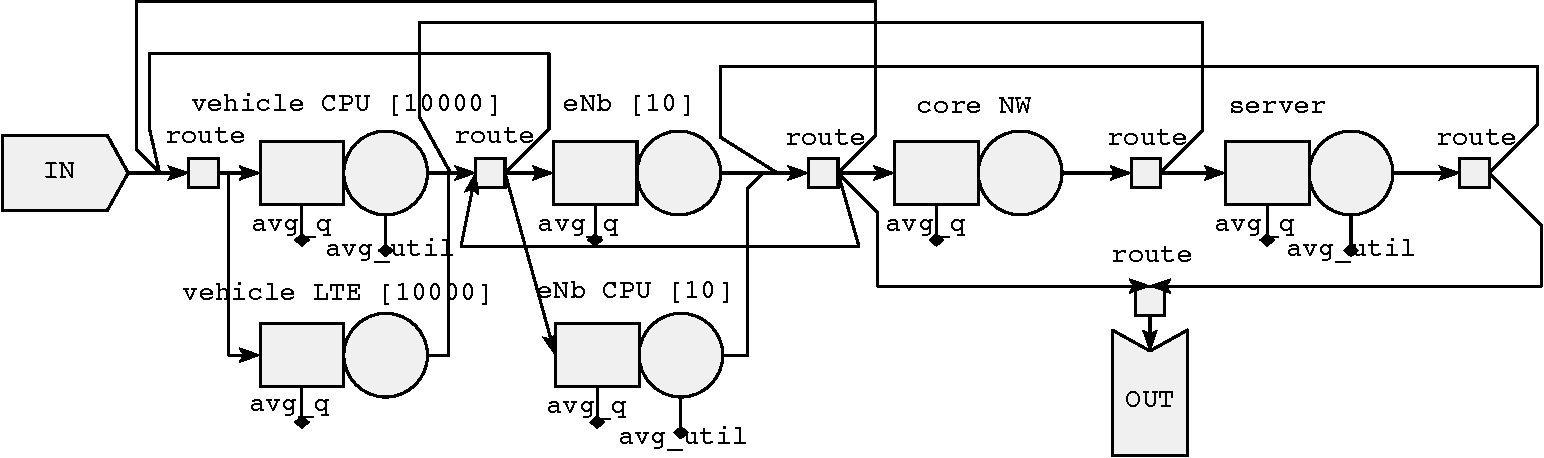
\includegraphics[width=\textwidth]{images/pse-rne-example-crop.pdf}
    \caption{An example of resource provision model.TODO: cite and add caption}
    \label{fig:resource-provision-model}
  \end{center}

\end{figure}

Figure \ref{fig:resource-provision-model} presents an example of a resource provision model ...
\todo[inline]{Explain the figure}

The resource usage models can be presented as message sequence charts or tasks graphs. We omit the discussion of the sequence chart in this thesis. Task graph is a presentation of the resource usage of the tasks arriving to the system. The nodes in the task graph can be divided into three categories: execution nodes describe the resource usage events and activities, branching nodes conditionally guide the tasks through the graph, and fork/join nodes present task subdivision. The arcs present the flow of control in the system.

\begin{figure}[]
  \begin{center}
    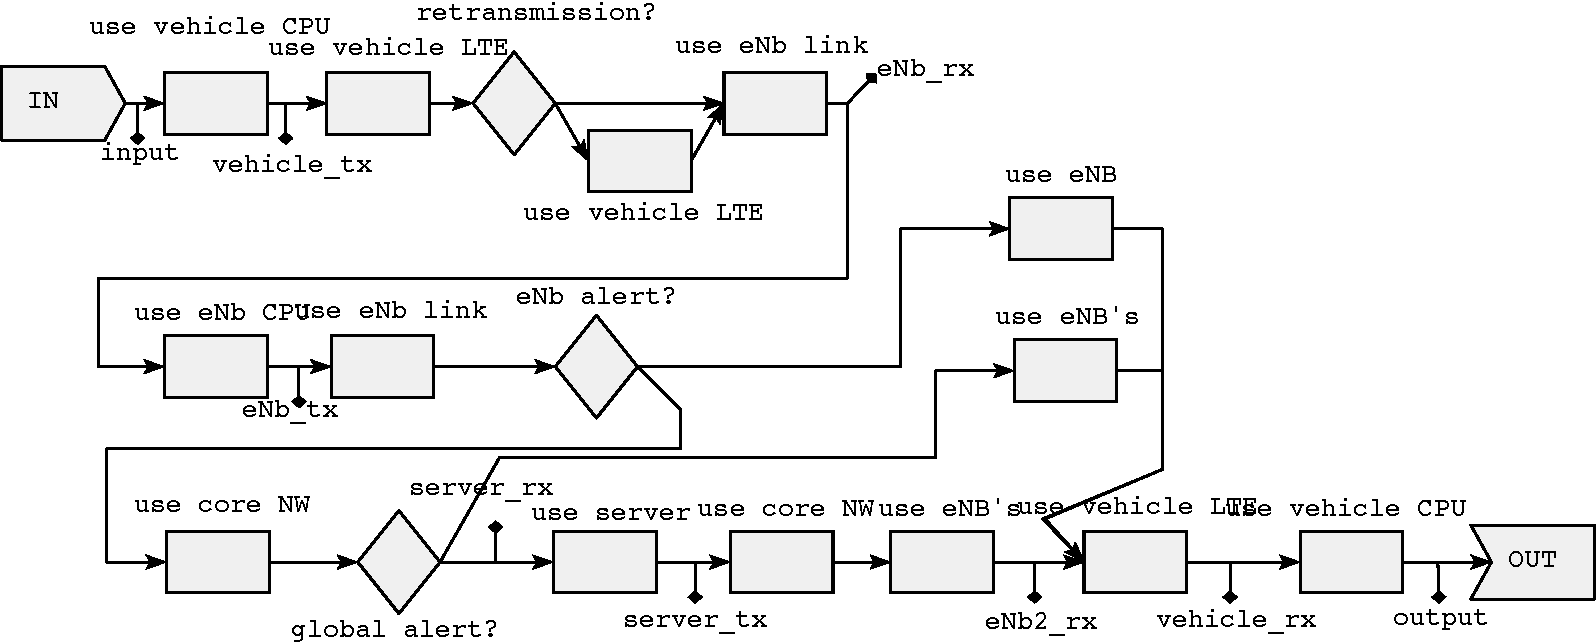
\includegraphics[width=\textwidth]{images/pse-tge-example-crop.pdf}
    \caption{An example of resource usage model.TODO: cite and add caption}
    \label{fig:resource-usage-model}
  \end{center}
\end{figure}

Figure \ref{fig:resource-usage-model} presents an example of a resource usage model ...
\todo[inline]{Explain the figure}

The workload model generates tasks, which traverse through the system according to the rules defined in the resource usage model, consuming the resources defined in the resource provision model. The nodes in the workload graph describe the task generating processes, and the arcs define the relationships between them. The graph representing the workload model must be acyclic.

The event spawn rate can be constant or random (specified for example with probability distribution).

When an event is spawned, it progresses through the resource provision model triggering the resource usages. -> gets delayed.

\begin{figure}[]
  \begin{center}
    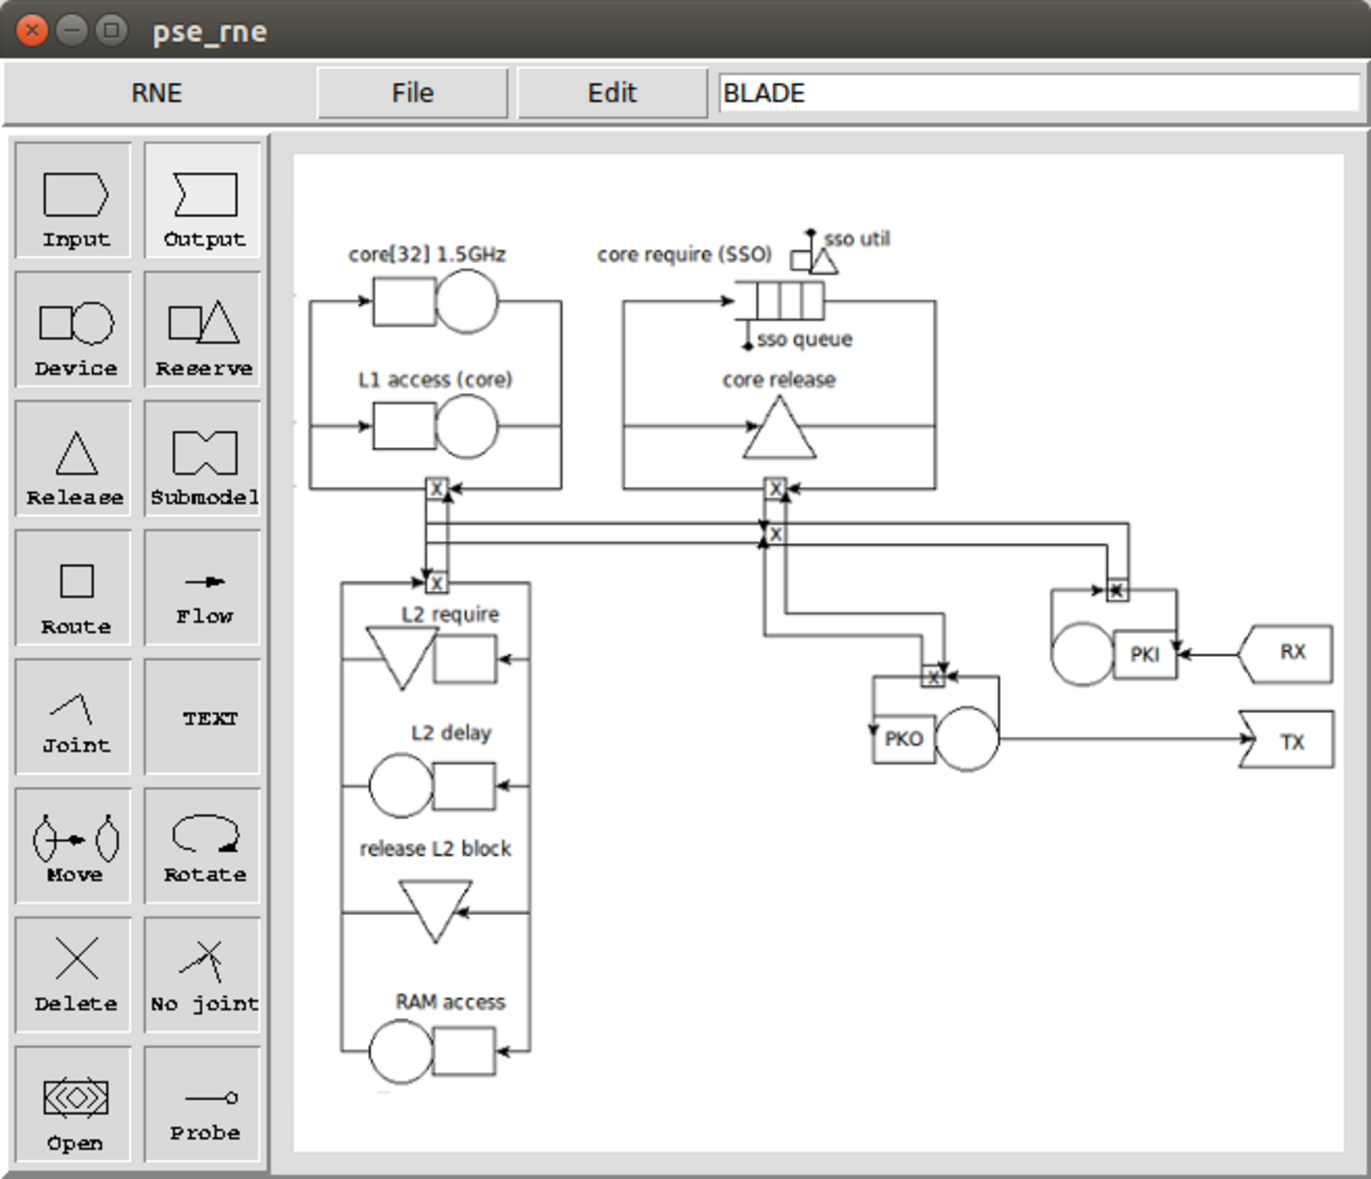
\includegraphics[width=\textwidth]{images/rne-example.pdf}
    \caption{The graphical user interface of the resource network editor. The actual resource network model is presented in the middle, and the toolbar on the left.}
    \label{fig:rne-example}
  \end{center}
\end{figure}

\section{Monitoring}

PSE has flexible, built-in, monitoring support which offers both trace-based and on-the-fly monitoring. The monitoring is controlled by attaching probes to the nodes and vertices of the simulation model nodes. It can be done on all the three model levels and practically every simulation system state change can be captured. There are essentially two different types of probes in PSE: the trace probes for trace-based measurements, and the metric probes for on-the-fly measurements.

In the resource provision model, the probes can be attached to two different parts of the resourse, to measure either the resource utilization, or its queue size. The trace probes capture every change in the resource utilization or queue size, whereas the metric trace produce aggregate only the descriptive statistics. The descriptive statistics currently include mean, standard deviation, mininimum, maximum, sum, and total number of tasks that passed through.

In the resource usage model, the probes can be attached to the model edges, producing a timestamped trace whenever a task travels the edge. The timing can be either absolute time with respect to the global system time, or relative to the process start time. The metric probes can be used to capture the average times of all tasks relative to the start of the process. Probes in the workload model are used to control the grouping of the resource usage and resource provision probes.

The probe output is written in a text file defined in the probe node attributes. The trace probes write the output in Comma-Separated Values~\cite{Shafranovic:2005:CSV} format, and the metrics traces write a standard descriptive statistics output. Using the trace based probing can substantially slow down the simulation, as the output files easily grow very large, slowing down the writes. Thus, whenever the complete trace log is not needed, it is recommended to use the metric based probing. Figure~\ref{fig:full-model} in section~\ref{sec:simulation-model} presents examples of probes attached to core-, memory- and SSO units in the hardware model as well as the in- and out- probes int the software model.

\section{Resource Network Simulator}
\label{sec:resource-network-simulator}

Performance Simulation Environment provides a discrete event simulator engine, named resource network simulator (RNS). The final simulator program is created by compiling the RNS runtime libraries together with the generated simulation model code. The simulator engine manages the simulation execution, i.e. tracks the global simulation time, schedules tasks and manages the system monitoring.

The simulator inputs are generated by the workload model, which spawns a new system thread for each generated input. The input can be either a control input or an actual workload task. The former of these are used for the simulation control, for example changing or resetting the simulation time or monitoring metrics. The latter are the actual task entities presented in section~\ref{sec:simulation-model}.

\subsection{Simulator Engine}
\label{sec:simulator-engine}

\begin{figure}[]
  \begin{center}
    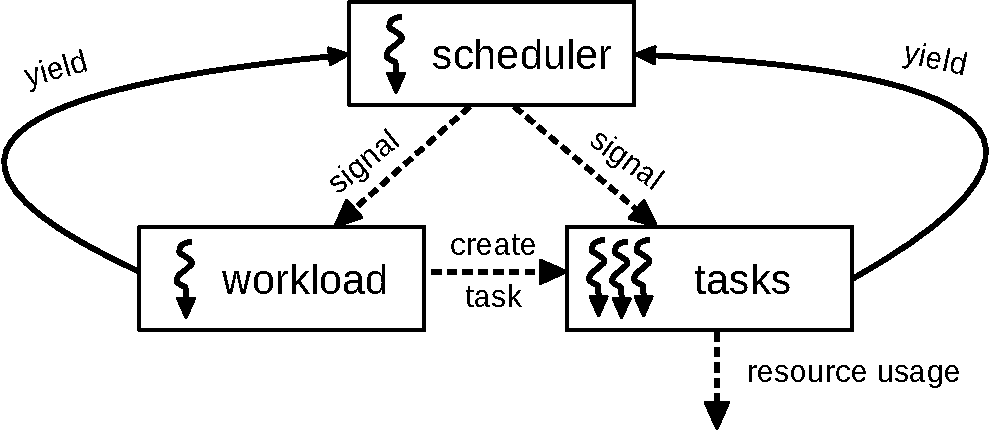
\includegraphics[width=\textwidth]{images/rns-threads-crop.pdf}
    \caption{The thread cycle of performance simulation environment's resource network simulator engine.}
    \label{fig:rns-threads}
  \end{center}
\end{figure}

Figure~\ref{fig:rns-threads} represents the model of execution in the RNS engine. The RNS scheduler, running in an infinite loop in its own thread, signals the workload threads or the task threads, based on the trigger time. RNS advances in the event-advance manner, meaning that the thread with the smallest trigger time, based on the scheduler's internal bookkeeping, gets always executed first.

The workload threads spawn new tasks to the actual taskpool, according to the code generated from the workload model. The execution of the taskpool threads advance the actual simulator, consuming the resources models based on the values defined in the resource usage model. Each time a thread's task encounters an event that is dependent on the other thread's execution, it yields the execution to the scheduler thread, which then signals the thread, again, with the smallest trigger time.

%%% Local Variables:
%%% mode: latex
%%% TeX-master: "thesis-hartikainen"
%%% End:


\chapter{Example Model of Packet Processing System}
\label{chapter:example-simulation-model}

\todo[inline]{make the use of terms packet, task, work, and event consistent throughout the text}
In this chapter, we present an example simulation model of Cavium OCTEON II CN6880 network processing unit~\cite{Cavium OCTEON}.

We will introduce the CN6880 hardware, and then describe the model components and entities of the simulation model, without diving into the details of the entity attributes. After that, we will go through the measurement setup required to obtain the reference values for the model. Two different measurements will be done, one to measure the communication latencies and another to measure the memory latencies. Then, the gathered reference values are plugged in to the model and describe the relevant details of it. Finally, we describe the implementation of the task scheduler, using the PSE plug-in interface

\section{Cavium OCTEON II CN6880}
\label{sec:cavium-octeon}

Cavium Octeon II CN6880 is a 32 MIPS core network processing unit, optimized for high-performance, high-bandwidth, and low power consumption software-defined control-plane~\cite{control-plane} and data-plane~\cite{data-plane} applications.

CN6880 provides several hardware acceleration units for enhanced packet processing and minimized software development complexity. The packet management accelerators offload the actual packet processing cores from many general packet receive, buffering, buffer management, flow classification, quality of service, and transmit processing. The accelerator functions can be customized using software, and accessing the configuration registers.~\cite{cavium:2010:fundamentals}

The packet input processor unit (PKI) and input packet data unit (IPD) work together to manage the received packets, and to perform required processing before scheduling the packets to application cores. They automatically handle most of the processing requirements of the layer 2 to layer 7 open systems interconnection model~\cite{OSI model}. Once the required computation is done, the PKI unit sends the packet's work entry to the SSO unit to be scheduled for processing.~\cite{cavium:2010:fundamentals}

The packet transmission is handled by the packet transmission unit (PKO). When a core finishes a packet processing, it notifies the PKO that the packet is ready for transmission. The PKO then directly copies the packet data from the shared memory into its internal memory, optionally computes checksums for the packet header, transmits the packet, and optionally frees the packet data from the memory.~\cite{cavium:2010:fundamentals}

One of the key features of the CN6880 is its scheduling/synchronization and order unit (SSO). It frees the actual packet processing applications, running on the 32 MIPS cores, from the complex packet scheduling and ordering tasks. The cores execute a loop, and when a core is ready for the next packet, it requests work from the SSO, which then schedules the next work based on the quality of service priority and work group.~\cite{cavium:2010:fundamentals}

The SSO also provides efficient locking mechanisms for protecting the critical regions without explicit software locking, and allows packet processing to be done in parallel or atomically, while still maintaining the packet flow order. The processing cores can also be dedicated for specific flows. One of our goals is to be able to model the scheduling functionality with PSE, as it is crucial to the packet latency and throughput when processing several flows at the time.~\cite{cavium:2010:fundamentals}

The memory latencies have large effect in the packet processing times. The CN6880 provides several memory policies for optimized multi-core packet processing. Each of the 32 cores have dedicated L1 data and instruction cache, and a shared L2 cache. The L1 data cache provides a hybrid write-through, write-back policy, using a write buffer mechanism, and the L2 cache implements a write-back policy. Several other cache related features are offered, for example to avoid unnecessary data writes after the packet transmission, and to automatically send the received packet header to L2 cache and the packet data to main memory, bypassing the L2 cache.~\cite{cavium:2010:fundamentals}

\section{Characteristic Measurements}
\label{sec:characteristic-measurements}

For the model to represent the packet latencies and throughput with enough accuracy, the model needs to be filled with apposite entity parameters. Some of model parameters are simple enough to be obtained directly from~\cite{cavium:2010:fundamentals}, while others are either unavailable, or are presented in a form unsuitable for our simulation model. The missing parameters are obtained by conducting measurements on the real CN6880 hardware.

% We believe that, by determining the latecies of input phase and output phase, the behaviour of memory, and modeling the packet scheduler with enough accuracy, the sought applications' effects to the packet latencies and throughput come up with enough accuracy.

% For our approach to be valid, i.e. the abstraction of the communication latencies to be precise enough, we have to assume the fastpath is not the bottleneck in the processing phase. This assumption is reasonable because ...

% \fixme{
%   TODO:
%   \begin{itemize}
%   \item because the fastpath hardware is optimized for this task
%   \item find reference
%   \item maybe justify the stuff with some kind of rough back-of-the-envelope calculation?
%   \end{itemize}
% }

\subsection{Communication Latencies}
\label{sec:communication-latencies}

The input and output phase latencies are measured by generating traffic from external machine, and passing it through two CN6880 units back to the generator itself. The measurements were done at two independent points in the processing path, to validate the accuracy of the measurements.

\begin{figure}[]
  \begin{center}
    \tikzstyle{block} = [draw, rectangle, thick, minimum height=2em, minimum width=2em]
\tikzstyle{dot} = [circle, inner sep=0pt, minimum size=1mm, fill=black,draw=black]
\tikzstyle{connector} = [->, thick]
\tikzstyle{line} = [thick]

\begin{tikzpicture}
  \small
  % node placement with matrix library: 5x4 array
  \matrix[ampersand replacement=\&, row sep=0.2cm, column sep=0.4cm] {
    \node[block] (l1) {External Traffic-Generator}; \& \& \&
    \node[block] (c1) {Forward Blade}; \& \& \&
    \node[block] (r1) {Swap Blade}; \& \\
  };

  %% Traffic gen probes
  \node [dot] (ld1) at ($(l1.10) + (0cm, 0.4cm)$) {};
  \draw [line] (l1.10) -- node[] {} (ld1);

  \node [dot] (ld2) at ($(l1.-10) + (0cm, -0.4cm)$) {};
  \draw [line] (l1.-10) -- node[] {} (ld2);

  %% Forward blade probes
  \node [dot] (cd1) at ($(c1.18) + (0cm, 0.4cm)$) {};
  \draw [line] (c1.18) -- node[] {} (cd1);

  \node [dot] (cd2) at ($(c1.-18) + (0cm, -0.4cm)$) {};
  \draw [line] (c1.-18) -- node[] {} (cd2);

  %% Swap blade probes
  \node [dot] (rd1) at ($(r1.157) + (0cm, 0.4cm)$) {};
  \draw [line] (r1.157) -- node[] {} (rd1);

  \node [dot] (rd2) at ($(r1.-157) + (0cm, -0.4cm)$) {};
  \draw [line] (r1.-157) -- node[] {} (rd2);

  %% Arrows connecting the nodes

  \draw [connector] (l1.7) -- node[] {} (c1.168);
  \draw [connector] (c1.12) -- node[] {} (r1.166);
  \draw [connector] (r1.-166) -- node[] {} (c1.-12);
  \draw [connector] (c1.-168) -- node[] {} (l1.-7);

\end{tikzpicture}

%%% Local Variables:
%%% mode: latex
%%% TeX-master: "../thesis-hartikainen.tex"
%%% End:

    \caption{The setup used to measure the communication latencies. The measurement points shown with the probes.}
    \label{fig:comm-setup}
  \end{center}
\end{figure}
\todo[inline]{Make figure \ref{fig:comm-setup} clearer, Emphasize the input and output parts of the flow.}

In figure~\ref{fig:comm-setup}, the rectangles represent three different computing units (traffic generator, forward unit, and swap unit), and the probes present the points of time measurements. The traffic generator is a typical desktop computer running Linux operating system, and the traffic was generated by Mausezahn~\cite{mausezahn}. Both of the CN6880 units are running Linux operating systems.

The packet is first generated at the packet generator and sent to the forward unit at time $t_{d0}$. Forwarding unit receives the packet, does the required processing and forwards the packet to the swap unit at time $t_{d1}$. The swap unit receives the packet at time $t_{r2}$, does the same processing as the forward unit (except with different destination address), and forwards the packet back to the forward unit at time $t_{d2}$. Finally the forward unit receives the packet at time $t_{r1}$ and forwards it to the traffic generator, which marks it received at time $t_{r0}$. The time $t_{f}$ spent in the input and output phase of one unit is then

\begin{equation}
  \label{eq:1}
  t_{f} = \frac{t_{r1} - t_{d1} - (t_{d2} - t_{r2})}{2}.
\end{equation}

We measured the times for packet sizes of 64B, 128B, 256B, 512B, 1024B, and 1500B, repeating the measurement for each packet 10000 times. Figure~\ref{fig:comm-latency} shows the resulting times $t_{f}$ for the different packet sizes.

\begin{figure}[]
  \begin{center}
    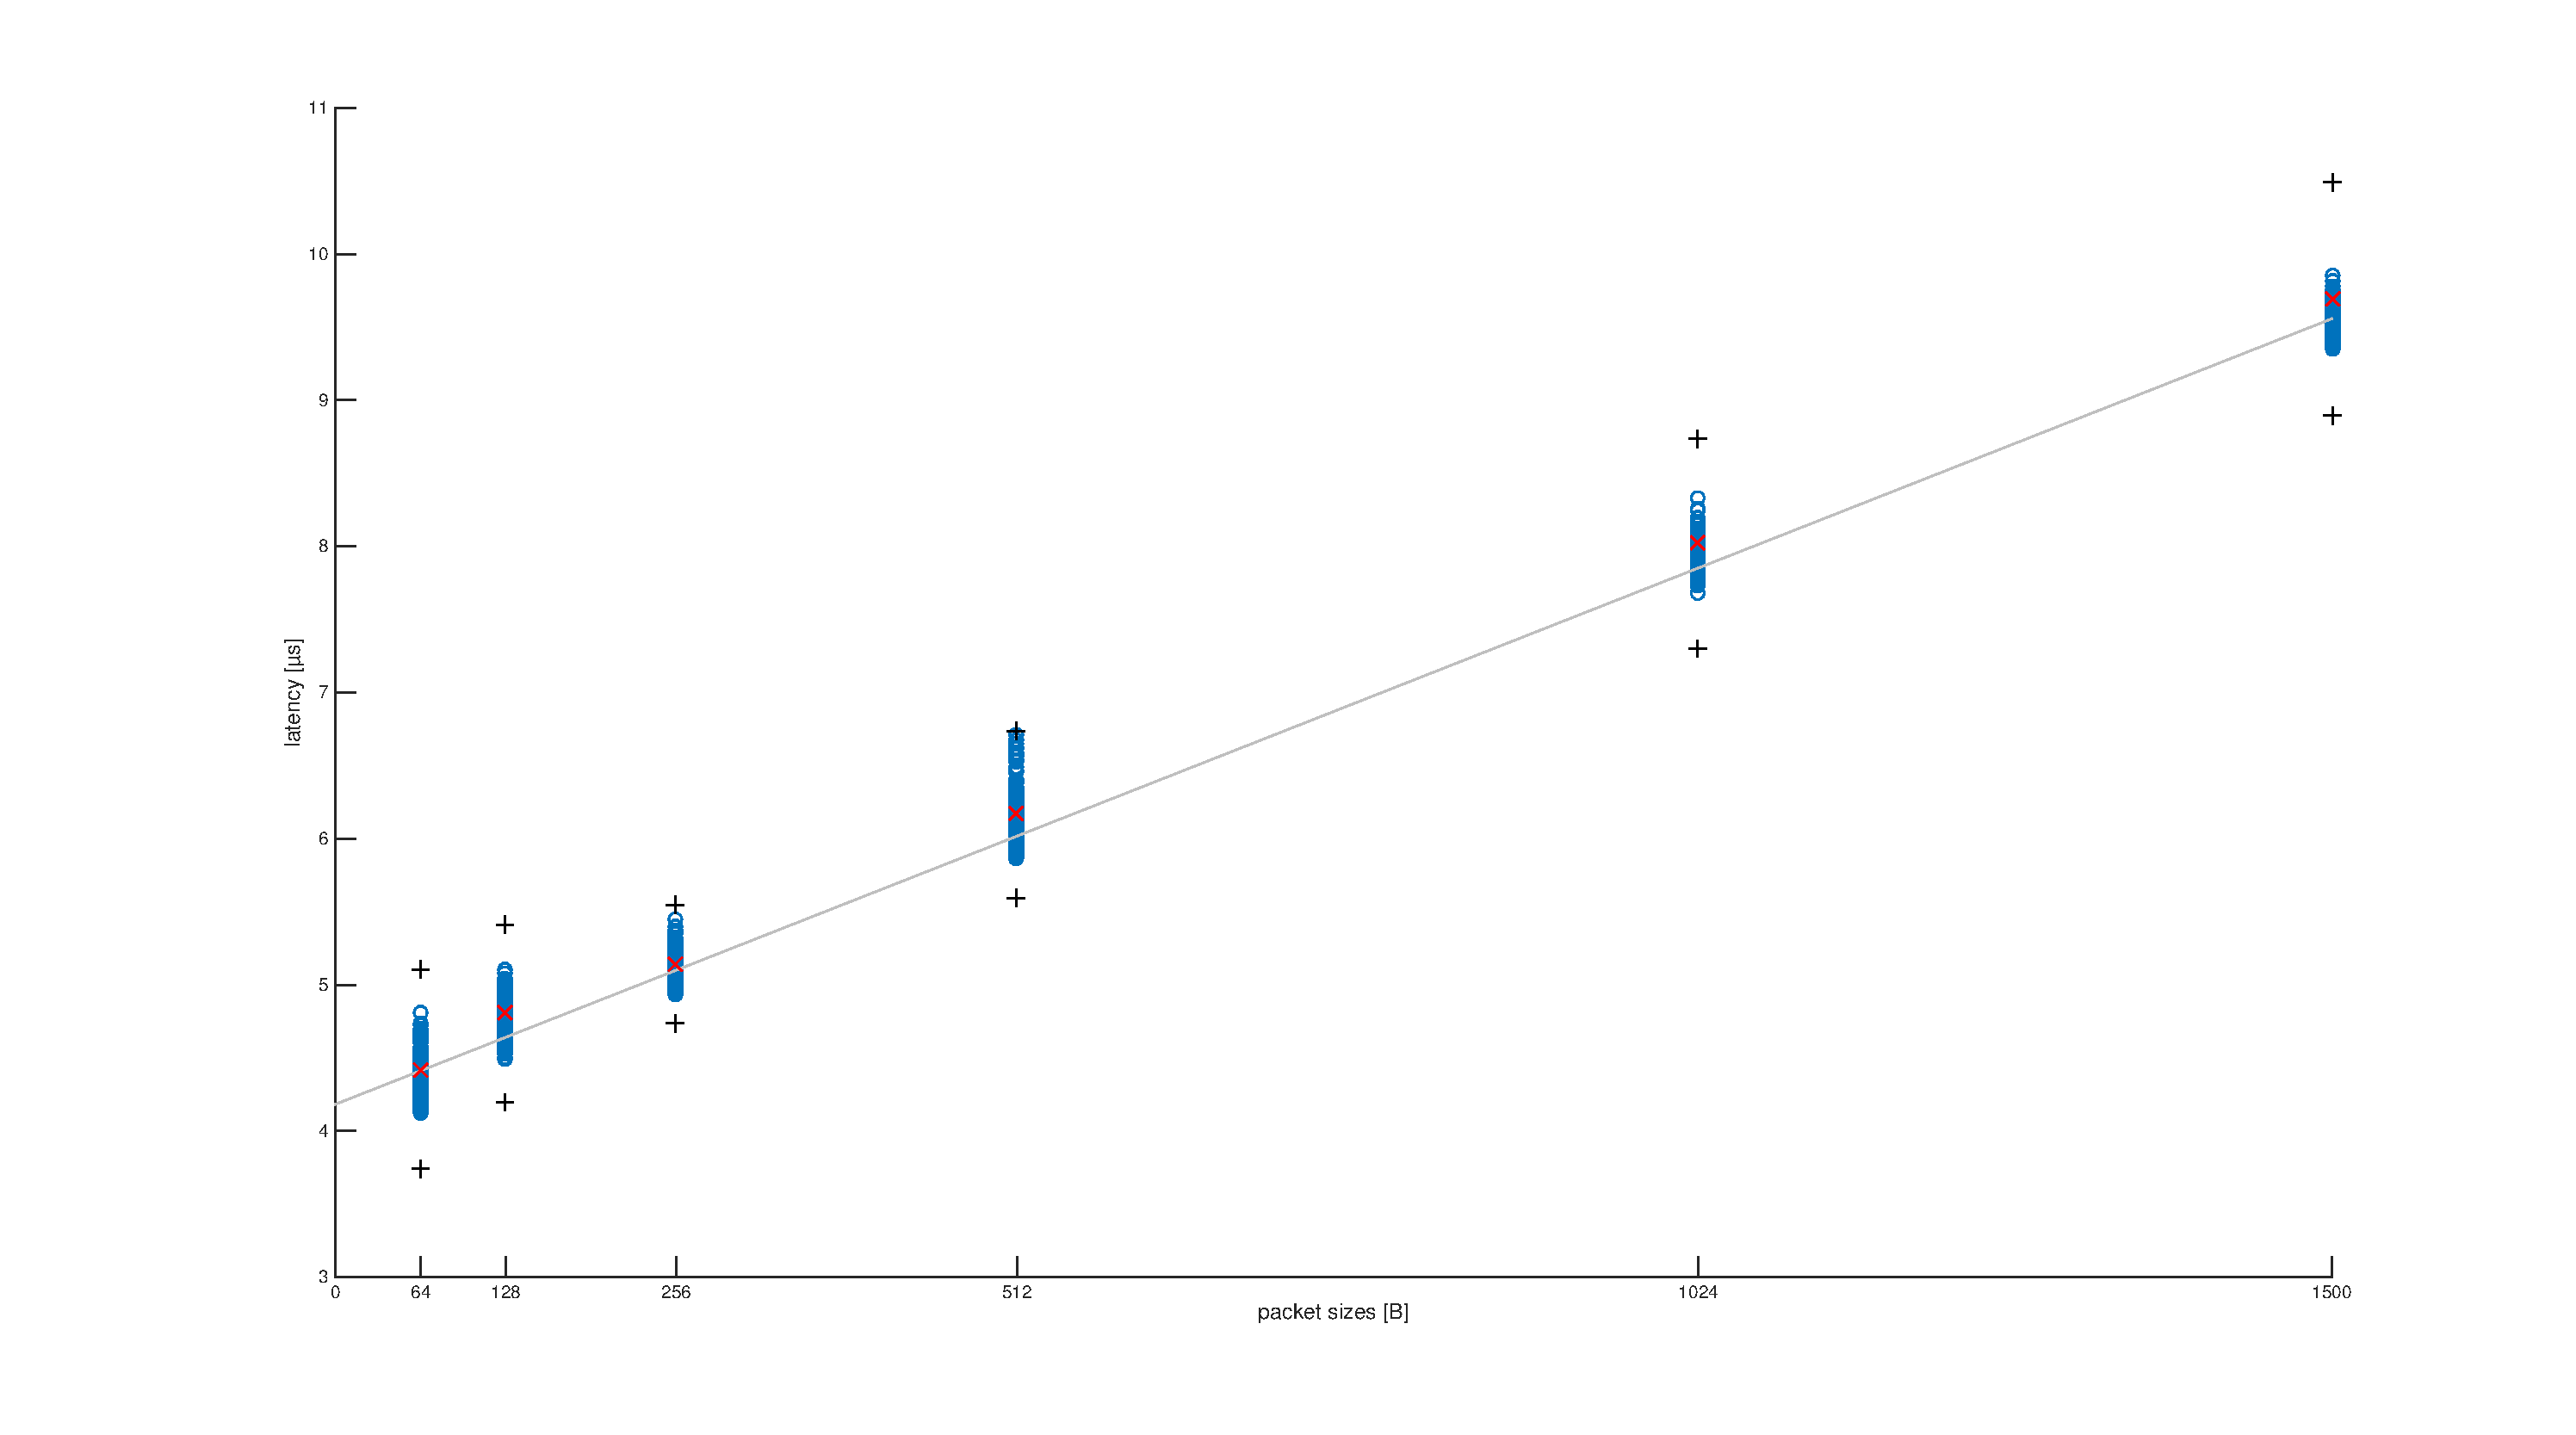
\includegraphics[width=\textwidth]{images/comm-latency.pdf}
    \caption{Latency of the input and output phase of the CN6880 unit. Averages marked as red X, and the 99\% confidence intervals with +. The trendline is of equation.}
    \label{fig:comm-latency}
  \end{center}
\end{figure}
\todo[inline]{check the confint}
\todo[inline]{latency = a*packetsize + constant}

As shown in the Figure~\ref{fig:comm-latency}, the time spent in the input and output phase of the unit is linear regarding to the packet size. The variation of the data is relatively small, and all the measurements correspond to the values measured with the external traffic-generator.

\todo[inline]{the following needs to be explained somewhere with the other fastpath stuff.}
\todo[inline]{Regardless of the packet size, the size of the work queue entry handled by the input/output units is the same.}
\todo[inline]{Also, the forward/swap code is constant in terms of packet size.}
\todo[inline]{Only operation that is dependent on the packet size is the copy from input to L2/RAM and from L2/RAM to output unit.}

As explained earlier\todo{actually explain this}, the only packet size dependent operations in the input/output phase are the  memory transfers between the memory (L2/RAM) and PKI or PKO.

We can not make a distinction between the input and output phase.
In our model, we will adjust the input/output phase amount so that they consume the PKI and PKO units for the amount that corresponds the constant term of equation \ref{eq:1}. The variable (non-constant) term is caused by the memory copies in the input/output phases, and are proportional to the packet size.

\subsection{Memory Delays}
\label{sec:memory-delays}

Memory delays were measured using Multi-core Processor Architecture and Communication (MPAC) benchmarking library. \cite{cite} Both, latency and throughput, were measured using for different dataset sizes and number of threads.

\begin{figure}[]
  \begin{center}
    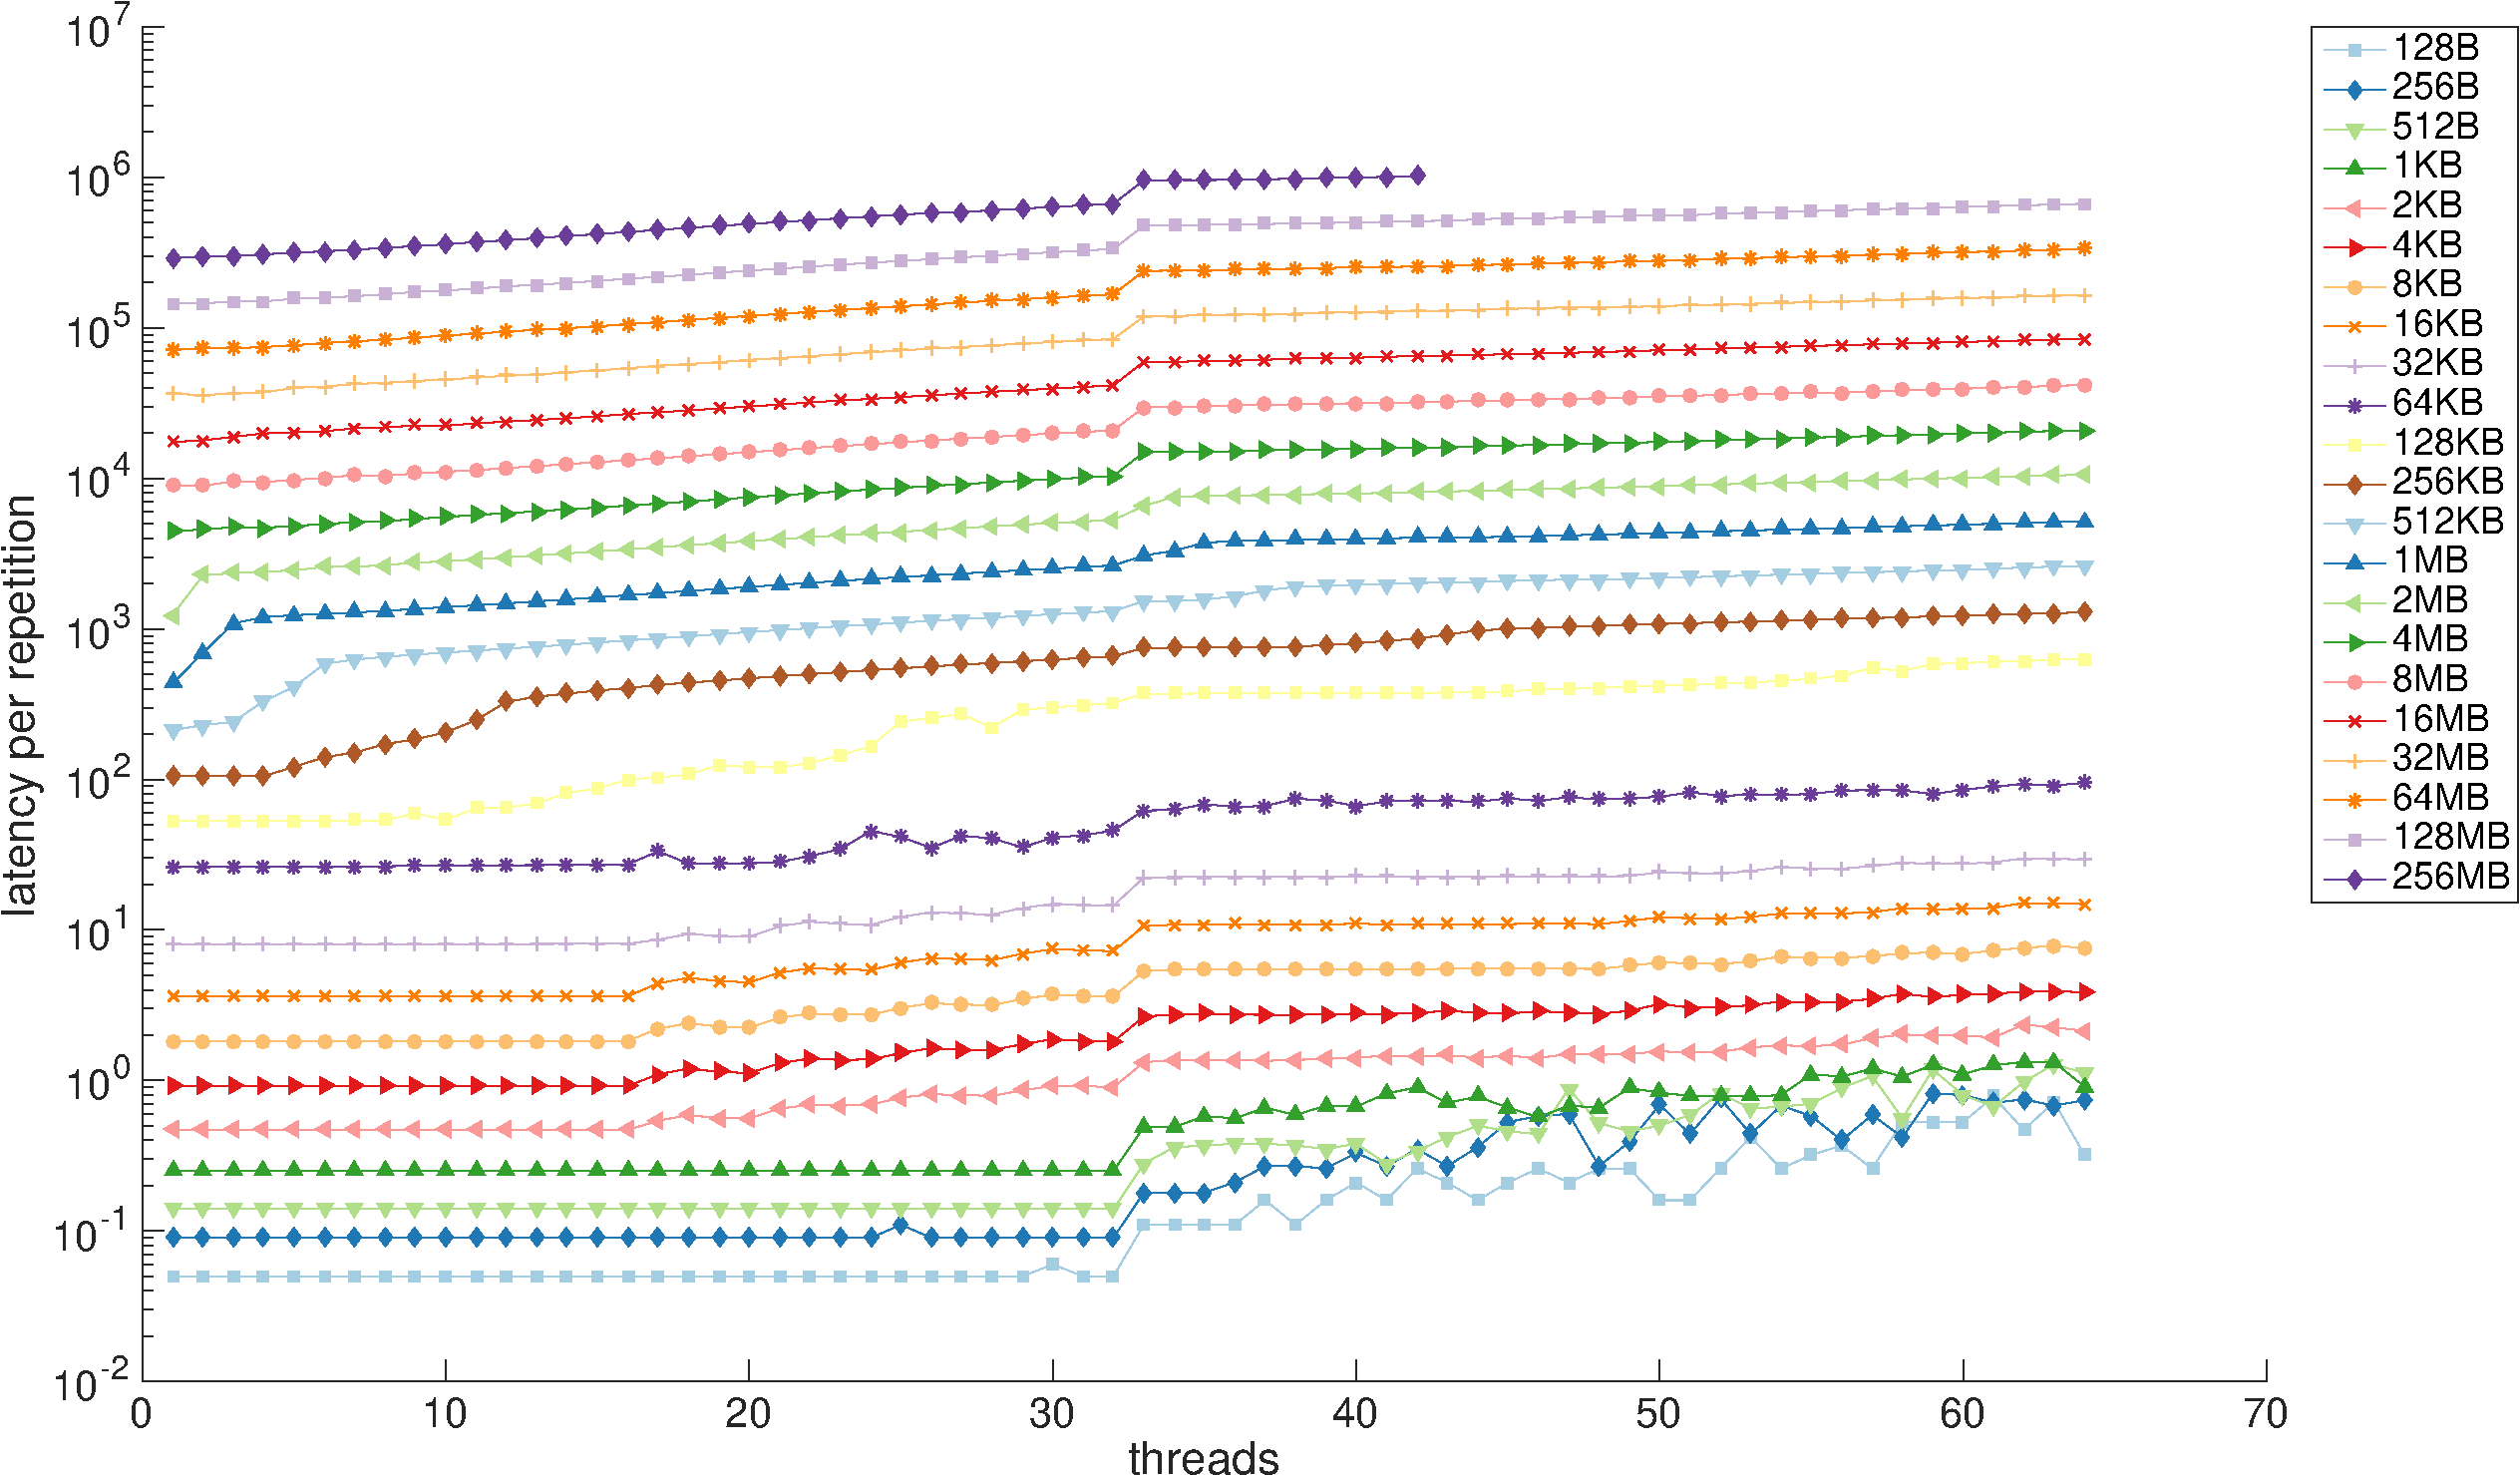
\includegraphics[width=\textwidth]{images/mem-latency.pdf}
    \caption{Memory latencies of the CN6880, measured by MPAC.}
    \label{fig:mem-latency}
  \end{center}
\end{figure}

\todo[inline]{logarithmic Y-scale}
\todo[inline]{explain the figure}

\begin{figure}[]
  \begin{center}
    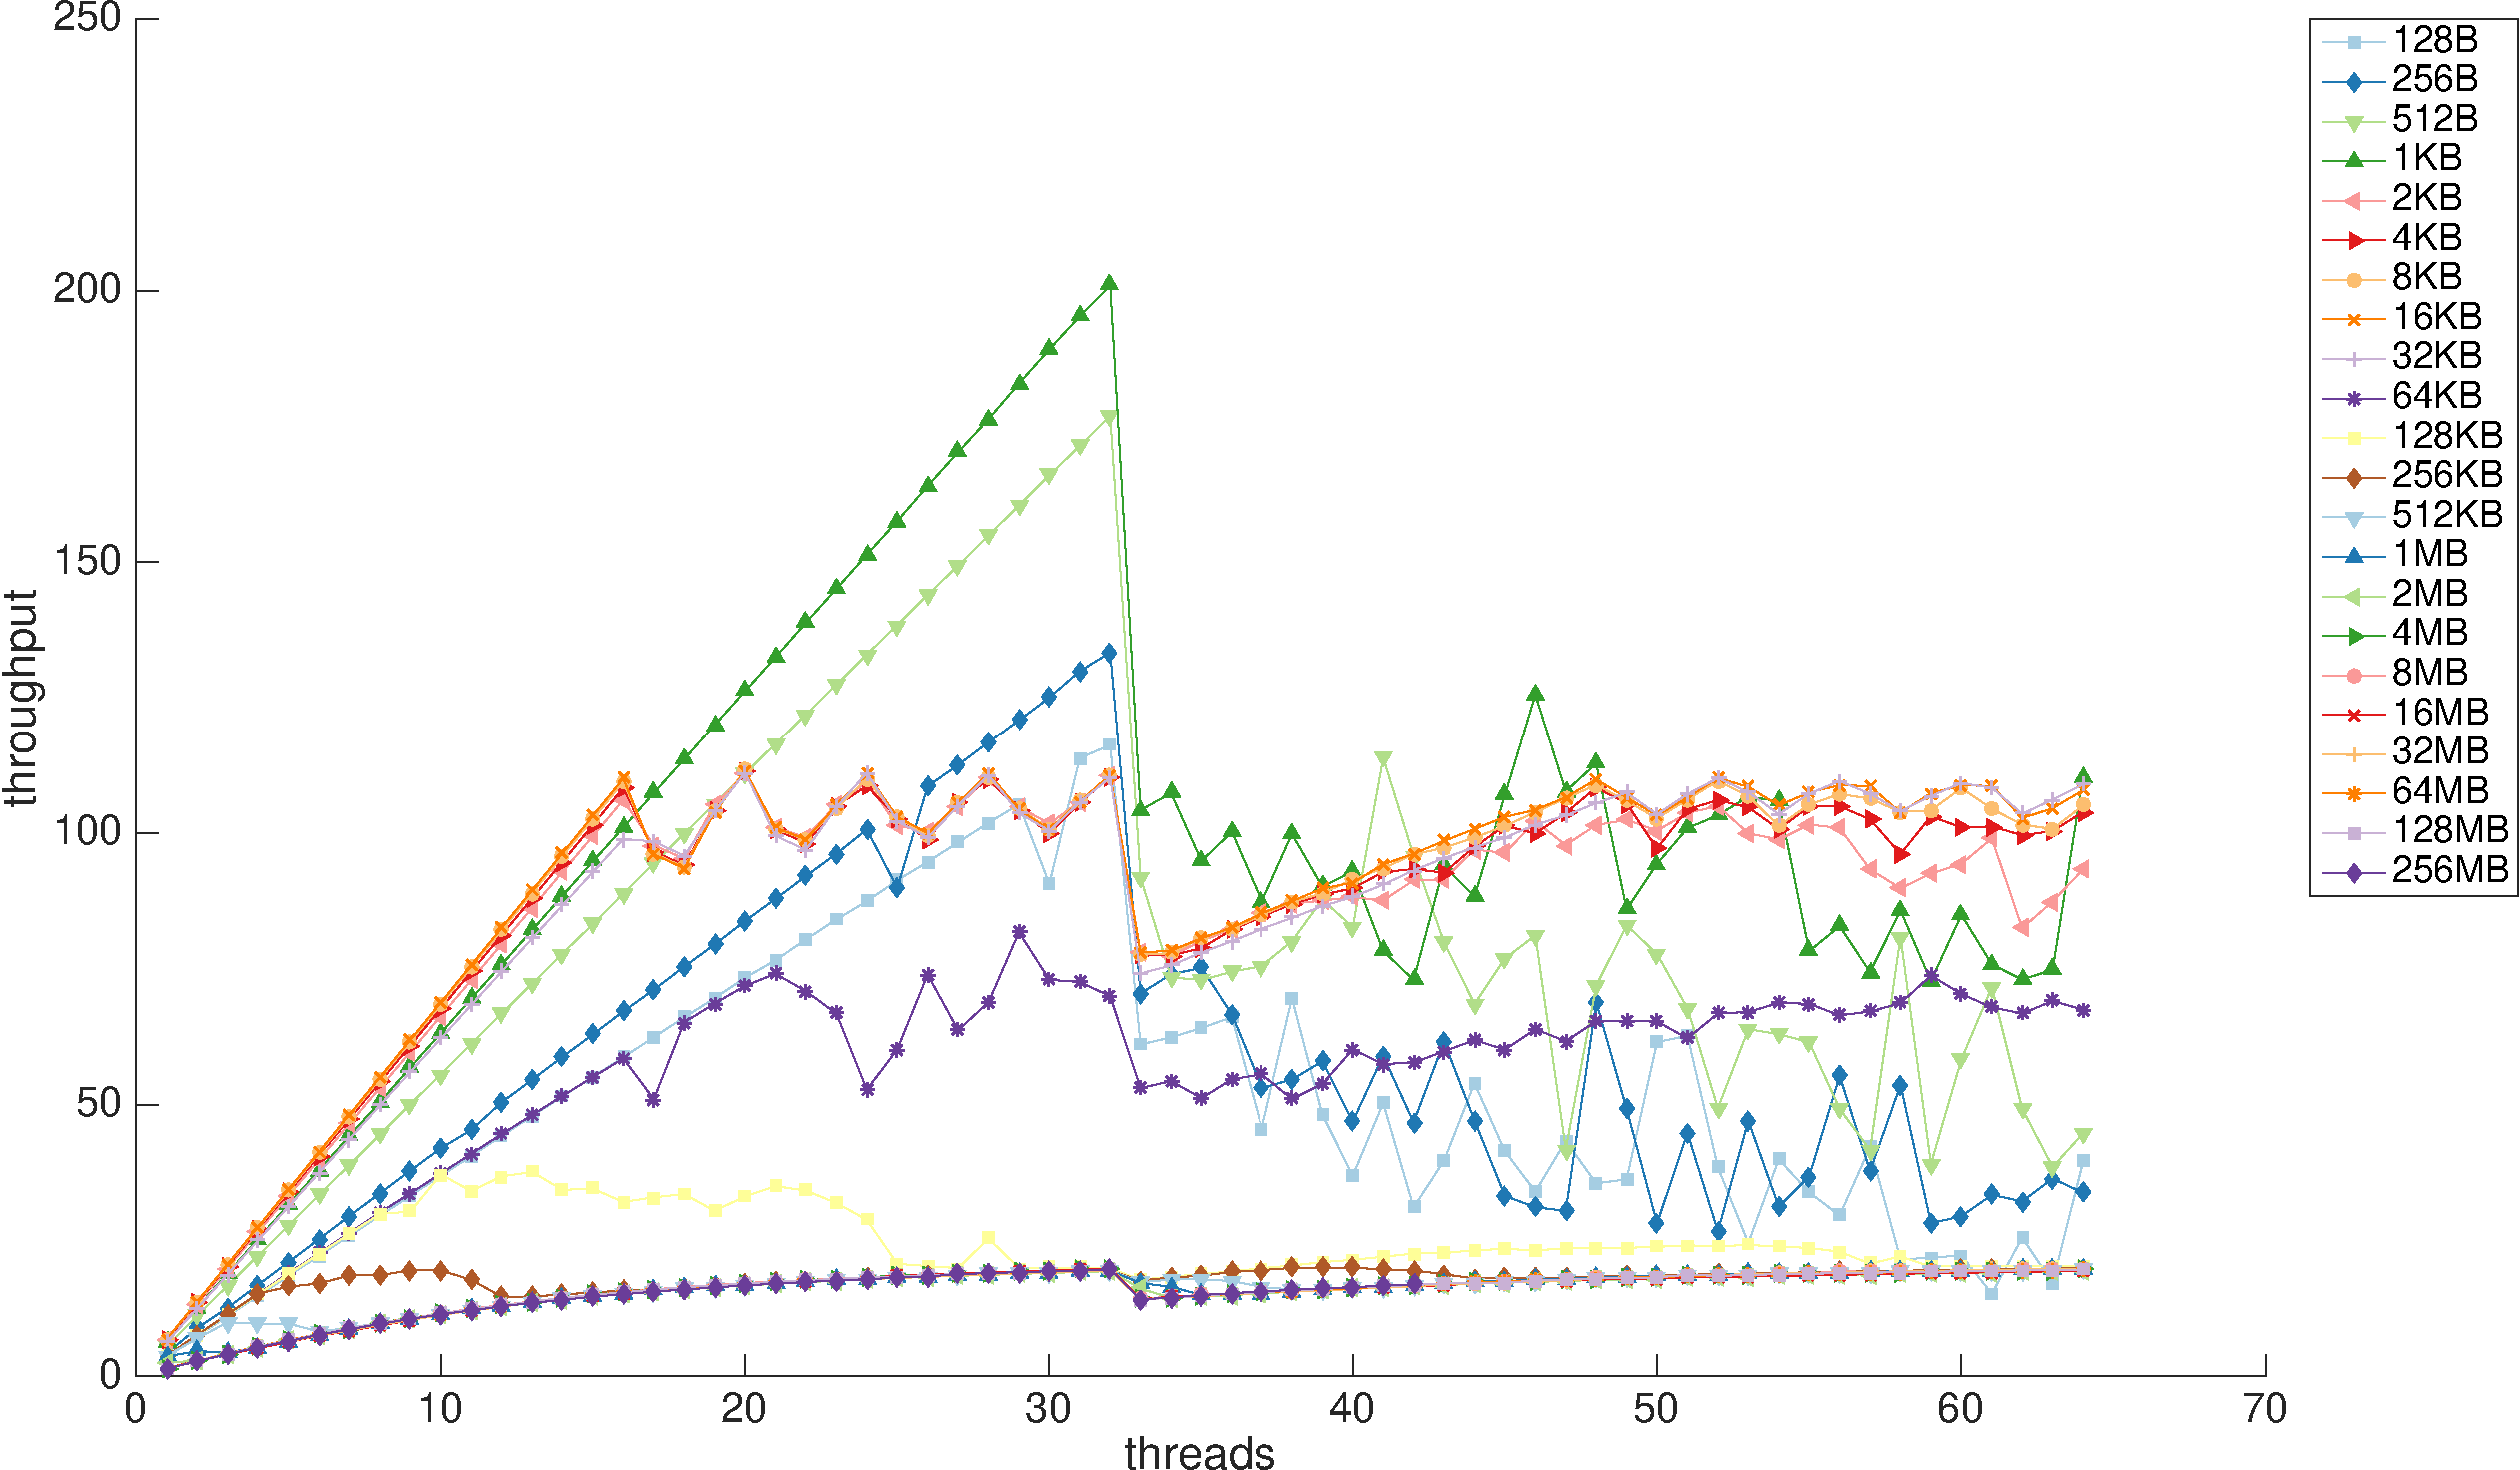
\includegraphics[width=\textwidth]{images/mem-throughput.pdf}
    \caption{Memory throughput of the CN6880, measure by MPAC.}
    \label{fig:mem-throughput}
  \end{center}
\end{figure}

\todo[inline]{explain the figure}

\section{Simulation Model}
\label{sec:simulation-model}

We created a simulation model of the Cavium OCTEON II CN6880 network processing unit with Performance Simulation Environment. The model is a high level abstraction of the real unit. As our interests are mainly in the applications' effect on the packet throughput and latency, we will not model the specific details of the hardware components. Figure \ref{fig:full-model} shows a layered representation of the main components of the model: workload, hardware, and software.

\begin{figure}[]
  \begin{center}
    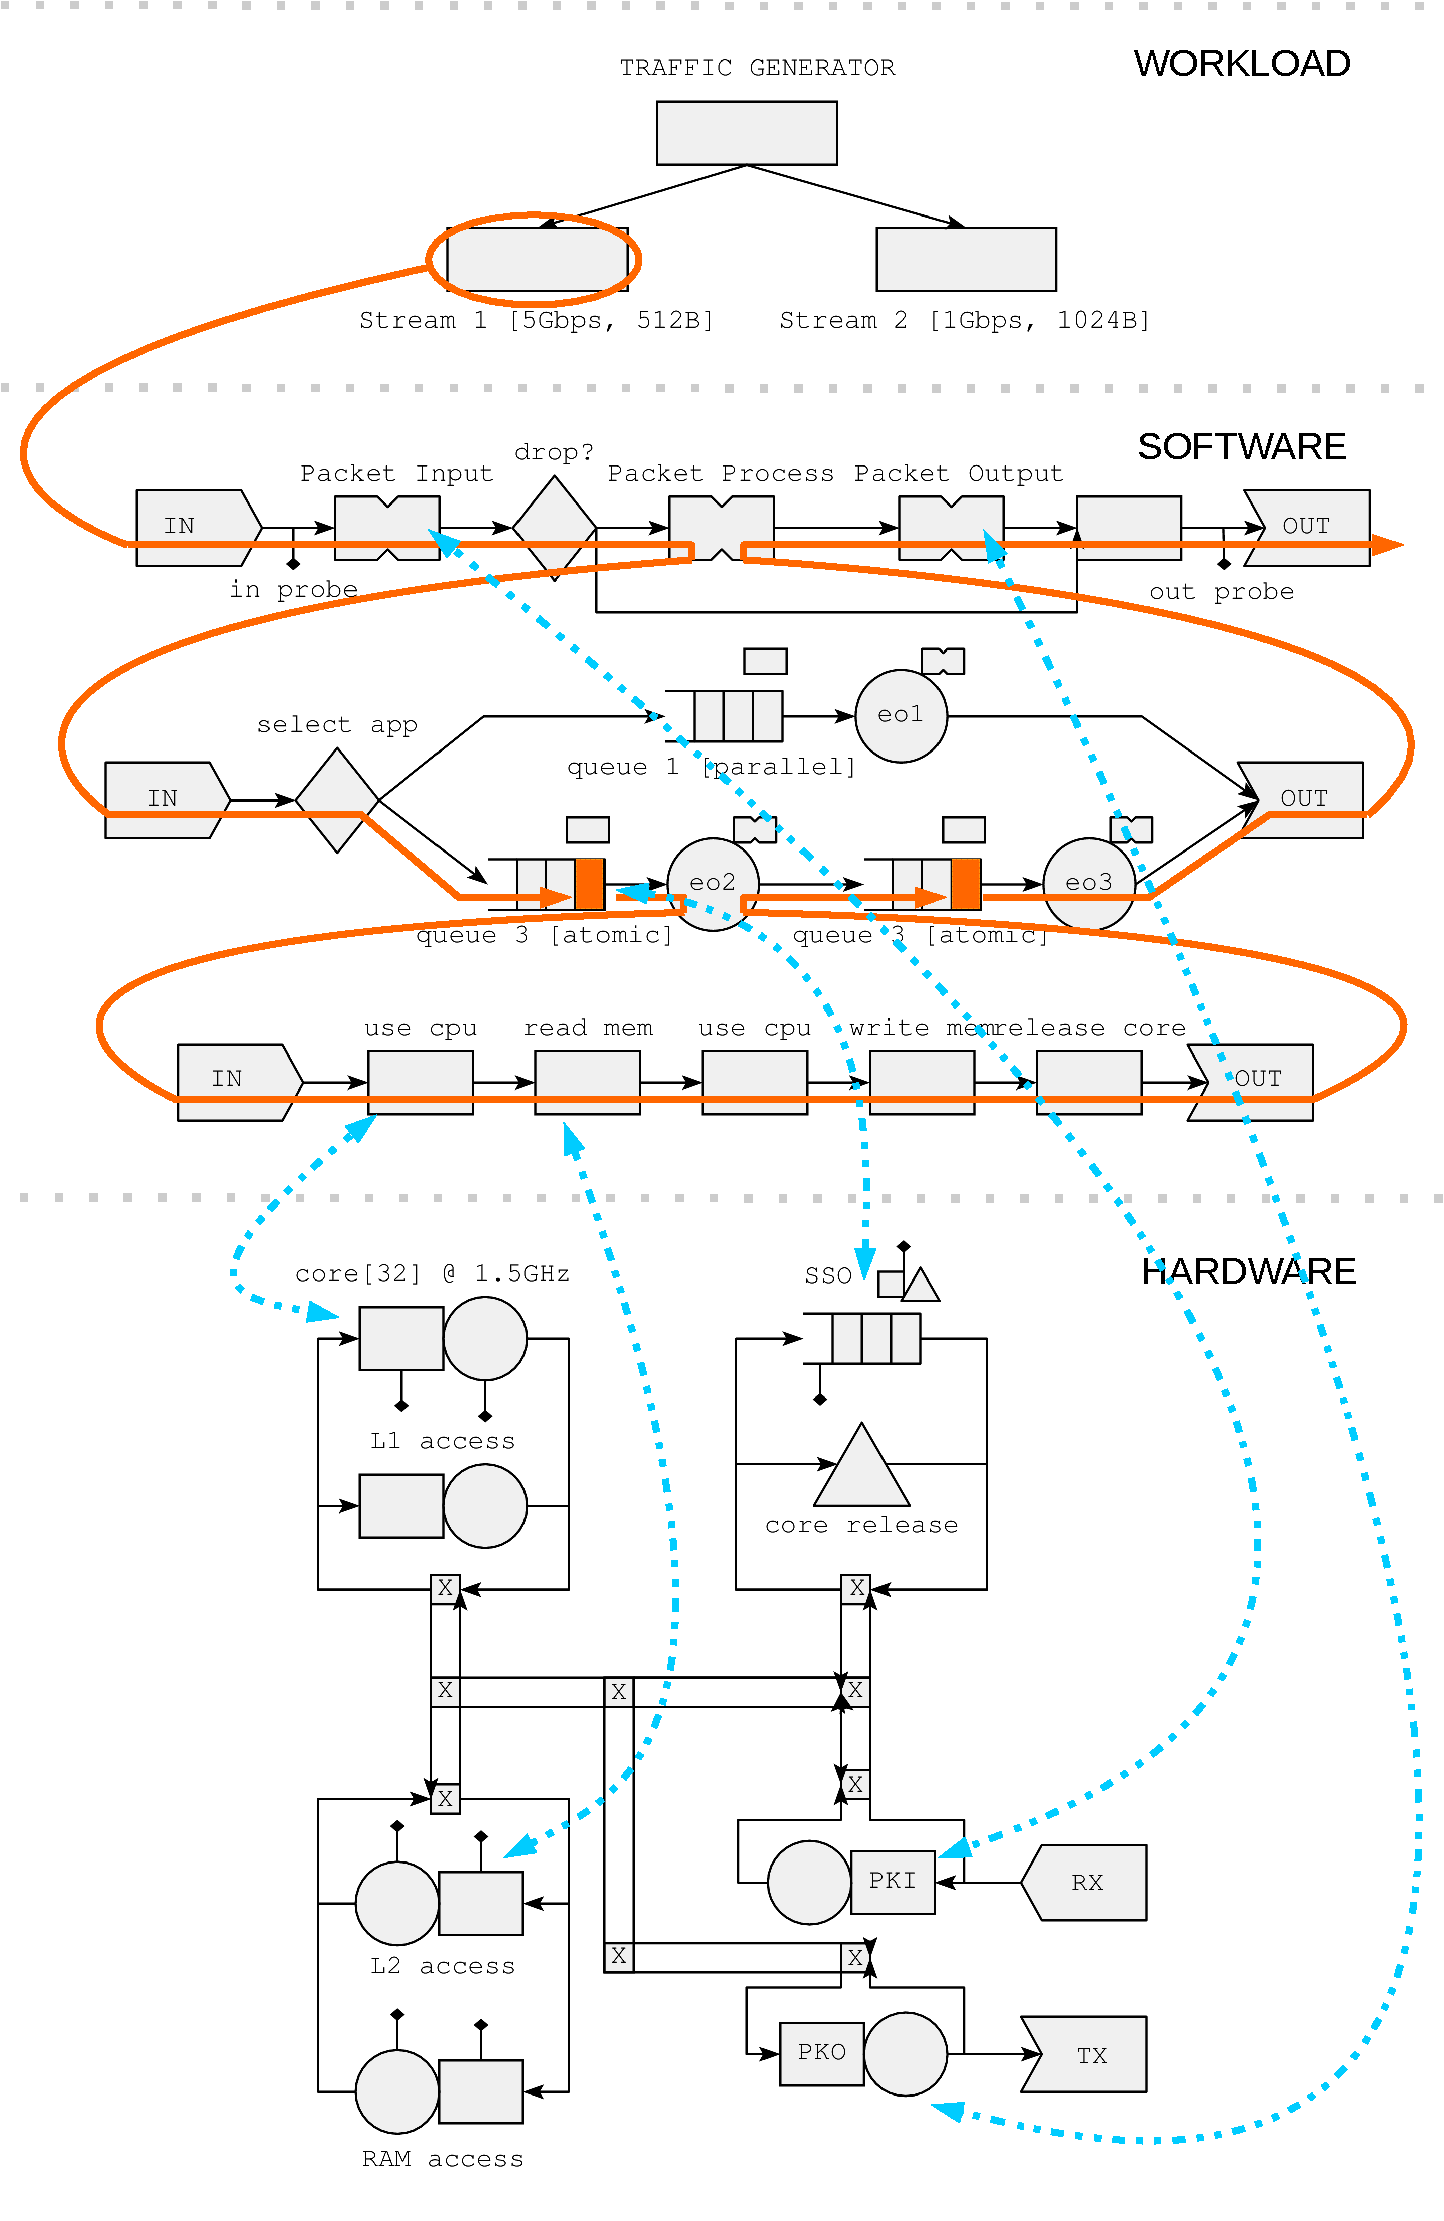
\includegraphics[width=\textwidth]{images/fullmodel-crop.pdf}
    \caption{Graphical presentation of the OCTEON II CN6880 PSE model. The workload model (top) generates network packets, which then flow through the software model (middle), consuming the hardware resources (bottom). The orange arrows represent an example of a packet's path through the software model, and the blue arrows the resource usage at each software model node.}
    \label{fig:full-model}
  \end{center}
\end{figure}

The workload model, at the top of the picture, consists of two packet streams. The TRAFFIC GENERATOR node activates the two stream nodes, which again generate packets that enter the software layer. The workload nodes contain parameters, such as the application id's, that are used to control the packet flows in the software model.

% has a lifetime of 0.5 seconds, and it triggers the streams with interval drawn from a uniform distribution with parameters 0.00005 and 0.00015. The streams have lifetime of 0.0004 seconds, and interval drawn from a lognormal distribution. The packet sizes of the streams are defined with the size attribute. Both of the streams also specify an appId attribute that is used to define the processing application in the software model. The packets from both streams enter the IN node of the top level software model.

The software model is divided into several submodels. The top software level model consists of packet input, packet processing and packet output submodels. The submodel view of the packet input and packet output are omitted from the picture for the sake of simplicity as in both of these phases, the core and memory usage is linearly dependent on the packet size, with additional Gaussian noise. In the input phase, the packet consumes specific amount of core cycles for the header processing, and copies the packet header and the packet data to the memory. Packet output node copies the packet from the memory, and consumes certain amount of clock cycles for the packet checksum calculations.

The packet processing submodel is presented in the middle software layer. The select app node forwards each of the packets to one of the two packet processing application, based on the application id attribute defined in the workload model. The queue nodes represent the core scheduling done by the SSO hardware unit. The packets arriving in the upper application have priority of 1, and they can be processed in parallel. In the application below, there are 2 atomic queues with priority 3. When the packet receives the passive resource from SSO, it can enter the actual processing application, called execution object (eo). The execution objects are submodels that consume core cycles and memory similarly to the packet input and packet output submodels presented above. The SSO/core passive resource is released inside each of the eo's.

The hardware model is a simple one level model containing no submodels. In the bottom left hand corner, there are PKI and PKO devices providing processor cycles for the packet input and packet output phases. The only passive resource node, SSO, provides core access resources, that can be released with the core release node. The application cores are shown in the top left corner of the hardware layer. There are 32 cores, and a specific L1 cache access for each of them. The L2 and RAM memory resources provide the delay for reading and writing to memory.

The probes, attached to the SSO unit, the cores, and the memory nodes, are used to gather statistics from the execution. Each of the units have two probes, one to measure the resource usage, and the other to measures the queue for the corresponding resource. In this hardware model, the routing nodes (squares) and the edges connecting the resources do not have any functional meaning, but are used solely to mimic the graphical models of the CN6880 unit presented in~\cite{cavium:2010:fundamentals}.

\section{Modeling the Task Scheduler}
\label{sec:modeling-task-scheduler}

The Schedule/Synchronization/Order (SSO) unit has an important effect on the task throughput times, as it controls the order in which the task get service from the application cores. This section first describes the application nodes used to model the SSO unit, and then the actual plug-in functions used to implement the scheduling functionality on the hardware model level.

% The SSO unit assigns the tasks to the processing cores.

% SSO unit needs to have a global

% The SSO unit schedules the tasks for the cores based on the

% Modeling a task processing application

% Figure~\ref{fig:full-model} has two different task processing applications.

% Before the task can be processed, it must wait for the SSO to schedule it on the core.

% When modeling the applications on PSE, it is helpful to consider the flow from the task's perspective. When a task has passed the input processing, it is put into the SSO queue to wait to be scheduled on the application cores. Each time a core finishes its previous task, it requests for a new work from the SSO-unit, which then schedules a task based on the flow QoS priority and work group.

\subsection{Application Models}
\label{application-models}

Each packet processing application consists of two parts: the SSO queue node, and the actual processing. The software layer in Figure~\ref{fig:full-model} presents and example of two main applications. The second application is divided into two sub-applications. The parameters for the first application's queue and execution object are shown in the Listings~\ref{lst:queue-attributes} and ~\ref{lst:eo-attributes}, respectively.

\lstinputlisting[caption=The attributes of the SSO queue.,
                 label=lst:queue-attributes]{listings/queue-attributes.txt}

The first line in Listing~\ref{lst:queue-attributes} specifies the display title for the node, as shown in the Figure~\ref{fig:full-model}. The \emph{name} and \emph{type} attributes specify that the resource usage is passive, and the required resource provision entity is $core\_require$, i.e. the SSO. The parameters on lines 5-7 define the parameters that are used in the custom scheduling code on the hardware level. The \emph{$queue\_type$} value atomic specifies that two nodes entering the SSO from the same resource usage node, cannot be processed simultaneously. The \emph{$queue\_id$} is used to keep track of the tasks being processed, and \emph{$queue\_priority$} is used to globally prioritize tasks between the queues.

\lstinputlisting[caption=The attributes of execution object.,
                 label=lst:eo-attributes]{listings/eo-attributes.txt}

nThe execution object node parameters are shown in the Listing~\ref{lst:eo-attributes}. It is a simple submodel node. It specifies the display title, and the name of the submodel to be used. The \emph{file} attribute specifies the file that defines the submodel. Note that, each execution object submodel needs to release the SSO/core resource, as shown in the Figure~\ref{fig:full-model}.

\subsection{Custom Scheduler Functions}
\label{sec:custom-scheduler-functions}

% Because the tasks processing in CN6880 is done in run-to-completion manner, the SSO unit is modeled as a passive resource. Each time when a tasks is entering a processing application, it must acquire the passive SSO resource. The amount of available passive SSO resources are equal to the processing cores in the system, and a task cannot use processing core without holding the SSO resource.

% The SSO scheduling is done in the SSO node presented in the hardware level in Figure~\ref{fig:full-model}. The actual scheduler function is written as a plug-in code, using the interface provided by PSE. The custom scheduling in PSE requires two functions, which are written in C-code: the selection function, and the reserve function. Each time a task enters a resource usage node in the task graph, the reserve function is called. The reserve function either

To model the SSO unit, a custom scheduling functions are required. PSE enables fully customizable resource scheduling through its plug-in interface. The actual scheduling functions are written in C-code, and the resource node parameters are changed to use these functions. The parameters of the SSO node used in the example model are presented in the Listing~\ref{lst:RNS-attributes}.

\lstinputlisting[caption=The attributes of the SSO node to determine the custom scheduler.,
                 label=lst:RNS-attributes]{listings/SSO-attributes.txt}

The first three lines specify the node title, name, and capacity. The capacity is set to the amount of available processing cores, meaning that no more than 32 tasks can be processed simultaneously. The \emph{discipline} parameter \mbox{CUSTOM}, on line 5, specifies that a custom scheduler is used instead of the built-in scheduling functions. The \emph{file} parameter specifies the path of the C header file that declares the scheduling functions. The \emph{$select\_function$} and the \emph{$reserve\_function$} parameters specify the two functions that are required to implement the scheduling logic.

The reserve function is called each time a task enters a resource usage node in the resource usage model, and it determines whether the task can immediately be served, or if it has to wait for the service. If the task can be processed immediately, it is inserted to the processing queue of the resource, and to the waiting queue otherwise. If the task gets put to the waiting queue, the reserve function also needs to reorder the queue.

Listing~\ref{lst:CUSTOM_reserve} describes the reserve function used to model the SSO. The function takes four input arguments: \emph{r} contains the data of the resource being reserved; \emph{queue} is a pointer whose value is assigned either to the processing queue or the waiting queue; \emph{position} is a pointer, whose value is assigned to the position in the queue; \emph{$new\_client$} holds the parameters, defined in the workload and resource usage models, of the new task.

\lstinputlisting[caption=The $CUSTOM\_reserve$ function for SSO.,
                 label=lst:CUSTOM_reserve]{listings/CUSTOM_reserve.c}

On the lines 11-39\todo{check the lines if the code changes!}, the reserve function attempts to place the task in the processing queue. The if-statement, on line 11, checks if the resource capacity is full. If there are available cores, then the processing conditions are checked, by going through all the cores, as shown in the for-loop on lines 21-32. If the new task's flow is marked atomic (in the reserve node in resource usage graph), and another task from the same flow is being processed on one of the cores (if-condition on lines 25-26), then the for-loop breaks, and the task gets set to the waiting queue. If a core is not processing, and the flow's coremask permits processing on the core (if-condition on line 31), we assign core's index to variable \emph{j}. Finally, if there is available core (\emph{j} is smaller or equal than the resource capacity) and none of the tasks from the same atomic flow are being processed, we set the queue to point to the resource's processing queue, and the position to the variable \emph{j}, and return.

If the processing conditions are not met, i.e. the execution goes past the if-block, then the task is set into the waiting queue. Line 43 assigns the \emph{queue} to point to the waiting queue of the resource. The for-loop on lines 46-48 finds the first task with larger priority, at index \emph{i}, and the for-loop on lines 51-53 moves all the higher priority tasks one step further on the queue. Finally the index \emph{i} is assigned to \emph{position}, and the function returns.

Each time a core ends a processing of a task, a new task is selected for the processing, using the the custom select function. Listing~\ref{lst:CUSTOM_select} shows the code used for the select function to model the SSO.

\lstinputlisting[caption=The $CUSTOM\_select$ function for SSO.,
                 label=lst:CUSTOM_select]{listings/CUSTOM_select.c}

$CUSTOM\_select$ takes the resource \emph{r}, and the index of the released core \emph{$release\_index$} as an input. The outer for-loop, starting at line 7, goes through all the tasks in the waiting queue, and finds the first task that satisfies the processing constraints, similarily as the reserve function. Line 10 checks if the waiting task's coremask allows the task to be processed on the core. If the waiting task's flow is atomic (line 12), we need to go through all the processing cores to check that there is no task being processed from the same flow (lines 18-24). If the task was not atomic, or no tasks from the same flow were being processed, the function returns the index of the task in the waiting queue. Otherwise we move to the next waiting task and repeat. If no task from the waiting queue can be scheduled, the function returns $RNS\_LARGE$. The RNS automatically moves the clients when it removes the task from the waiting queue.

%%% Local Variables:
%%% mode: latex
%%% TeX-master: "thesis-hartikainen"
%%% End:


\chapter{Demonstrative Experiment}
\label{chapter:demonstrative-experiment}

This chapter presents a demonstrative simulation experiment done on the CN6880 PSE model. The goal of the experiment is to demonstrate how the queue types and priorities affect the scheduler, and hence the packet throughput and latency, and at the same time validate the scheduler functionality implemented in the model. It also demonstrates the usage of probes to detect bottlenecks in a system.

\section{Experiment Setup}
\label{sec:experiment-setup}

The experiment consists of two different simulations and measurements. We will first demonstrate a packet processing application whose throughput is limited due to the bottleneck occurring from a slow atomic processing. We will then modify the application, splitting part of the atomic processing into parallel, thus breaking the bottleneck.

Both of the simulations consist of a single packet stream, which is generated from a two level workload model. The first workload node is similar workload generator node as presented in Figure~\ref{fig:full-model}. It triggers its child node with interval $RNS\_random\_uniform(5*10^{-5}, 15*10^{-5})$ seconds, and lifetime of 0.05 seconds. The child node creates 512B packets with interval $5.1~*~10^{-8}$~$*$~$RNS\_random\_lognormal(-10, 0.9)$ seconds for $4*10^{-5}$ seconds.

Figure~\ref{fig:experiment-hardware} presents the hardware model used in the experiment. It consists of six active resources. The PKI and PKO units are consumed by the input and output phases of the packet flow, respectively. Each 32 processing cores have a L1 cache associated with it, and the L2 cache and RAM are shared between the cores. The cores are served as first come first serve basis, as the scheduling logic is taken care of in the SSO unit.

The SSO unit uses the custom scheduling functions presented in the section~\ref{sec:custom-scheduler-functions}, enabling the use of atomicity, queue priorities, and coremasks. The core release is a typical relase node referring to the SSO unit.

\begin{figure}[]
  \begin{center}
    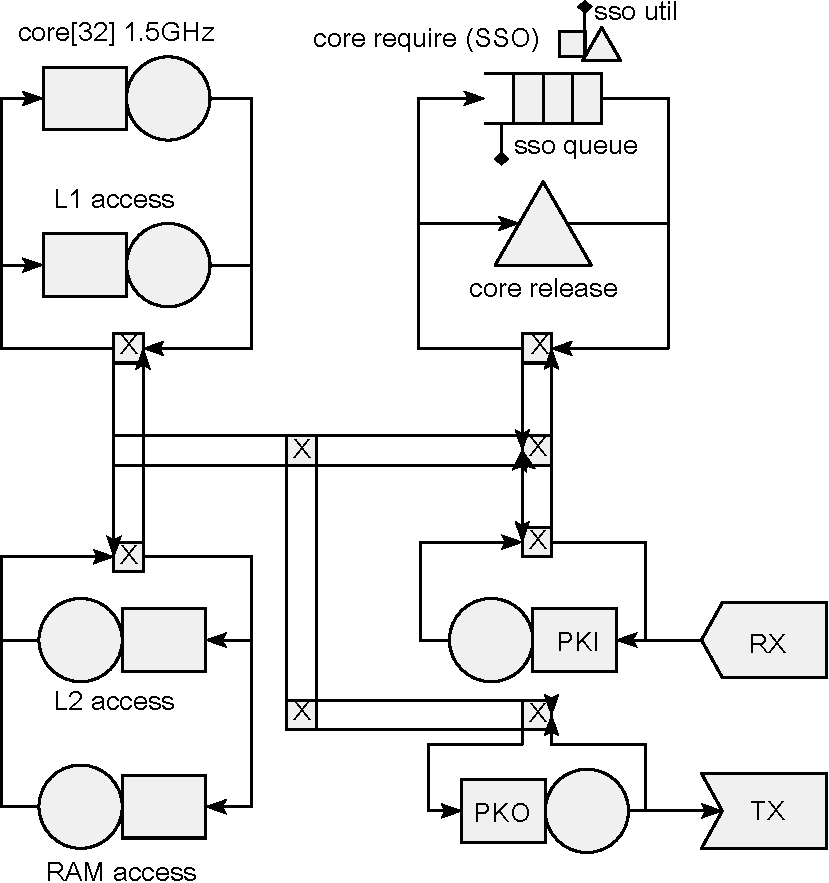
\includegraphics[width=0.6\textwidth]{images/pse-models/experiment-hardware.pdf}
    \caption{TODO}
    \label{fig:experiment-hardware}
  \end{center}
\end{figure}

The software model is presented in figure~\ref{fig:experiment-software}. The high level software model consists of the input, process, and output phases. The 'packet input' and 'packet output' nodes are modeled exactly as discussed in the section~\ref{sec:characteristic-measurements}, delaying the the packets according to the equation~\ref{eq:1}.

The two different applications used in the experiment, are shown in the software model after the 'select app' -node. The lower and upper application are referred as application 1 and application 2, respectively. The application selection is done in the workload model by the 'AppId' attribute.

The first packet processing application consists of two processing steps, both consuming CPU and memory for the range of 5000 clock cycles. The first step consists of parallel, priority 2 queue (A), and the second one is done atomically with priority 1 queue (B). The second simulation application is a modified version of the first packet processing application, where the second processing step is split into parallel and atomic steps. The release nodes are omitted from the software model for clarity.

\begin{figure}[]
  \begin{center}
    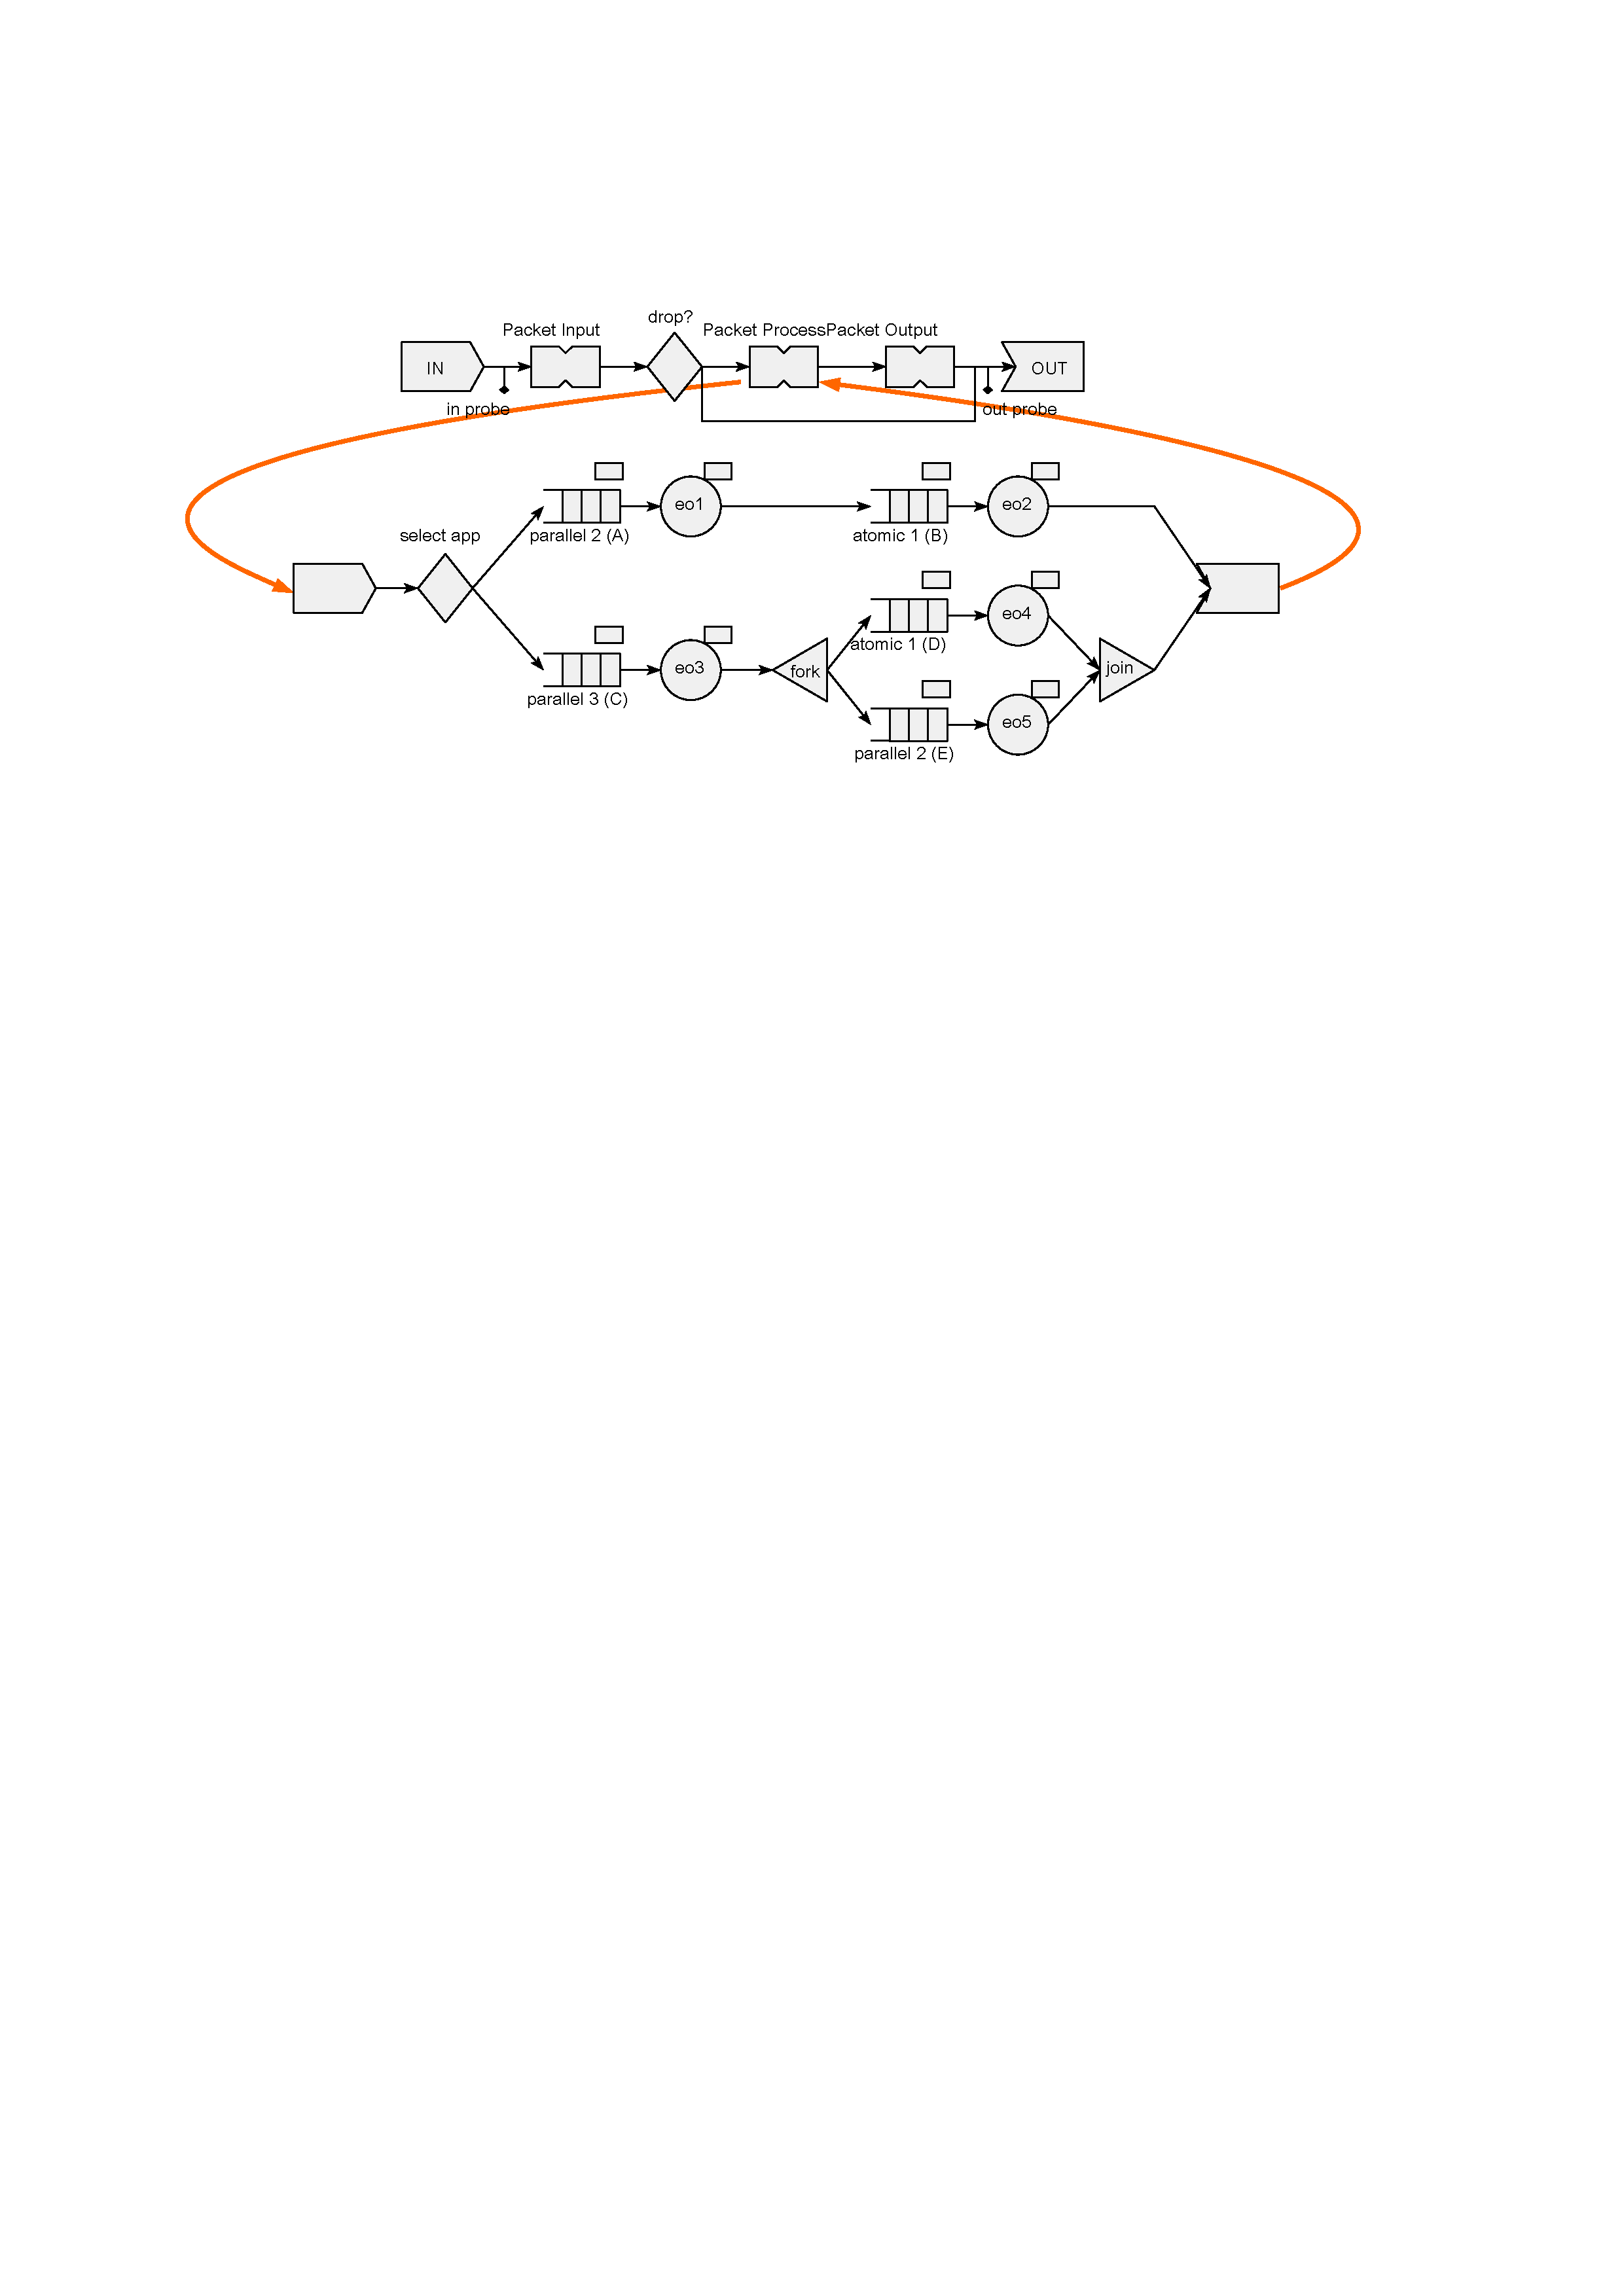
\includegraphics[width=\textwidth]{images/pse-models/experiment-software.pdf}
    \caption{TODO}
    \label{fig:experiment-software}
  \end{center}
\end{figure}

% \begin{figure}[]
%   \begin{center}
%     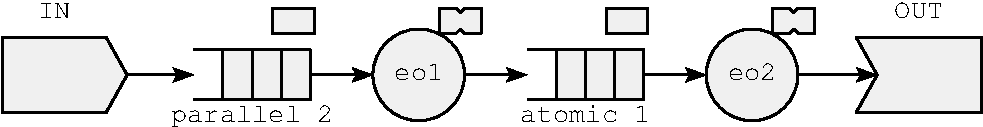
\includegraphics[width=\textwidth]{images/pse-models/application-1.pdf}
%     \caption{The example application used for the experiment. The atomic queue of eo2 produces a bottleneck to the system.}
%     \label{fig:application-1}
%   \end{center}
% \end{figure}

% \begin{figure}[]
%   \begin{center}
%     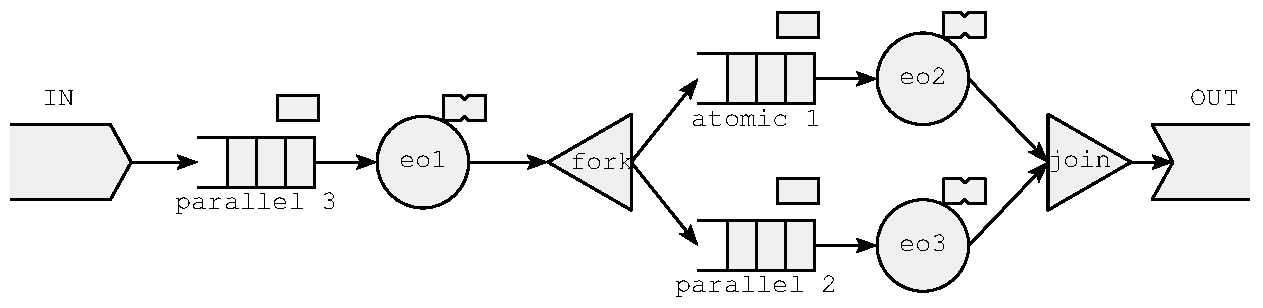
\includegraphics[width=\textwidth]{images/pse-models/application-2.pdf}
%     \caption{A modified processing application for the experiment. The bottleneck has been removed by splitting the second processing part into two.}
%     \label{fig:application-2}
%   \end{center}
% \end{figure}

We will gather two different metrics of the system. First, we are interested in the core utilization and queue lengths for each processing step. These are measured by the probes attached to the SSO unit as shown in hardware model in figure~\ref{fig:experiment-hardware}. Secondly, we are interested in the packet latencies. They are measured by calculating the time difference between the 'out probe' and the 'in probe', as shown in the software model in figure~\ref{fig:experiment-software}, for each packet.

\section{Simulation Results}
\label{sec:simulation-results}

The system was simulated twice, using both of the applications separately, and the data from the probes were post-processed. We grouped the number of tasks in the SSO/core queue, by the processing step.

Figures~\ref{fig:app1-queue2} and~\ref{fig:app1-latency} present the data from the first simulation using the packet processing application 1. Figure~\ref{fig:app1-queue2} describes the number of tasks in the SSO/core queue, that are from the atomic resource usage queue, with respect to simulation time. The corresponding graph for the first queue is omitted, as none of that tasks from it end up in the waiting queue. Figure~\ref{fig:app1-latency} presents the latency of each packet through the whole system.

\begin{figure}[]
  \begin{center}
    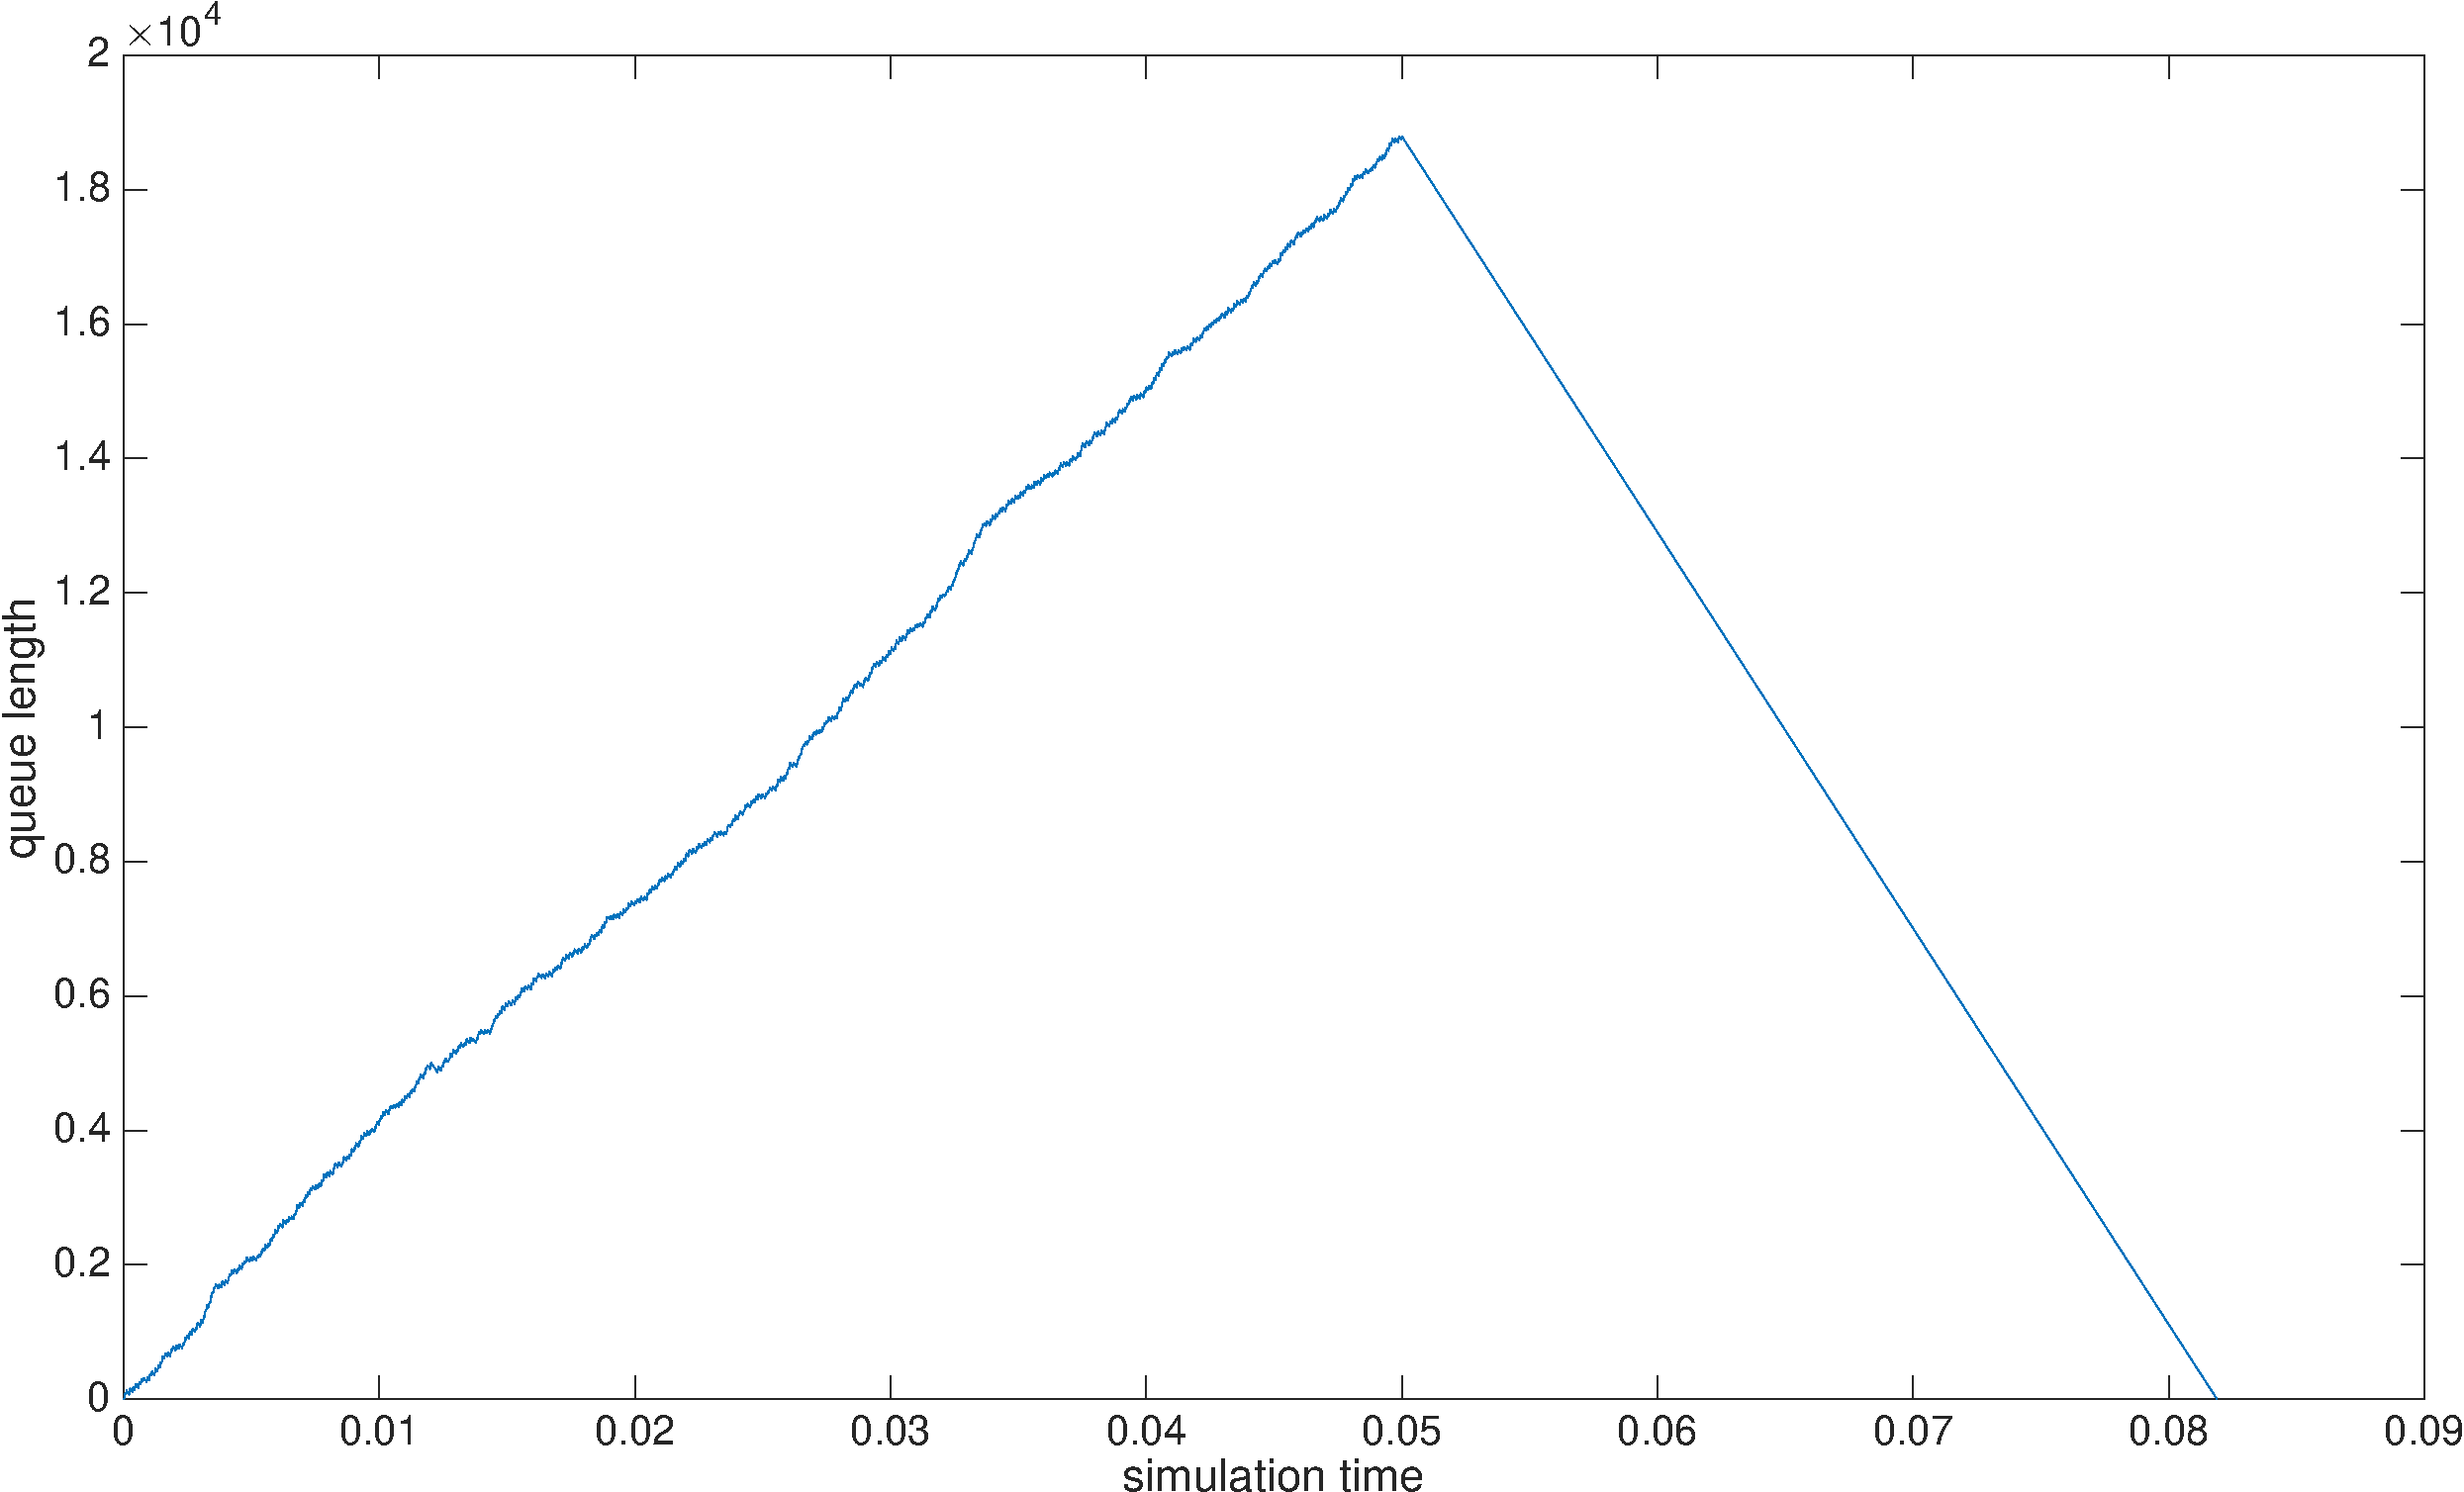
\includegraphics[width=\textwidth]{images/experiment/app1-queue2.pdf}
    \caption{Application 1: The number of tasks in the SSO/core queue, with respect to simulation time, from the second resource usage queue.}
    \label{fig:app1-queue2}
  \end{center}
\end{figure}

\begin{figure}[]
  \begin{center}
    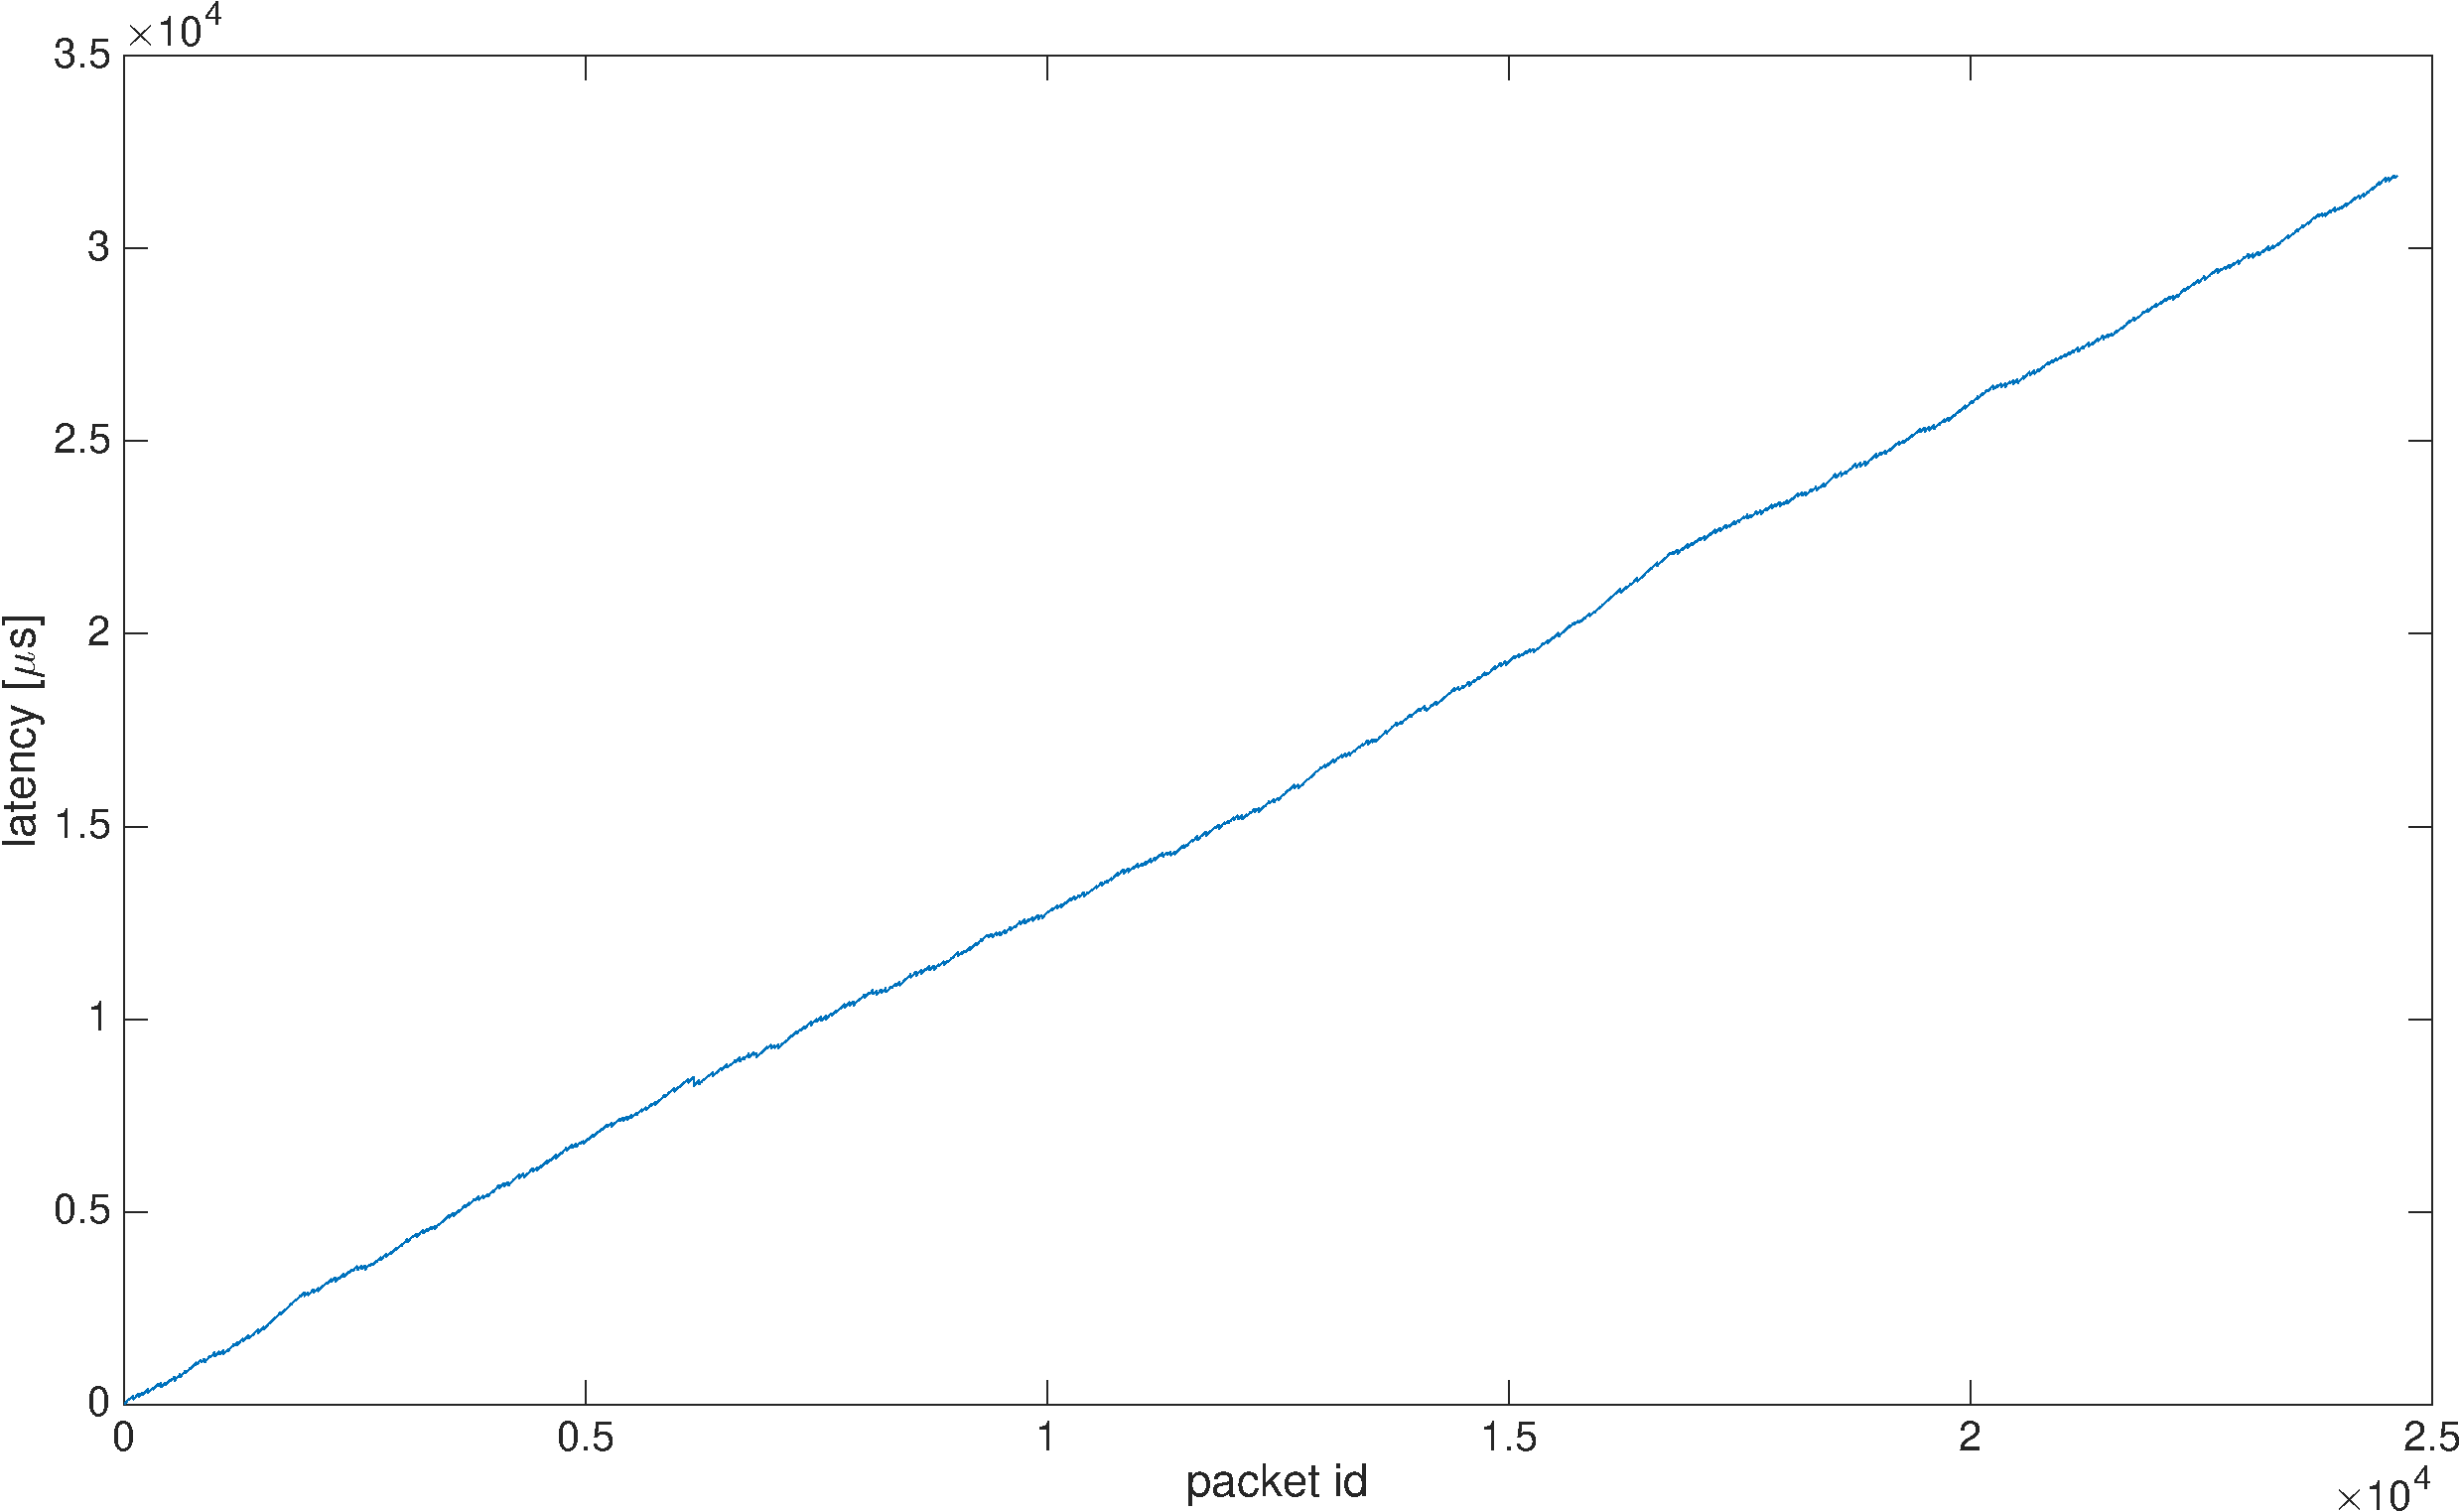
\includegraphics[width=\textwidth]{images/experiment/app1-latency.pdf}
    \caption{Application 1: Latency of the packets through the system.}
    \label{fig:app1-latency}
  \end{center}
\end{figure}

As shown in the figures, the second processing step produces a bottleneck to the system. The processing in the second execution object is so heavy that the tasks accumulate into the waiting queue, and thus the packet latency keeps growing until the workload ceases.

The second application removes this problem by parallelizing part of the atomic processing. Figures~\ref{fig:app2-queue2} and~\ref{fig:app2-latency} present the data from the second application simulation. Figure~\ref{fig:app2-queue2} shows the number of tasks in the SSO/core queue, that are from the atomic resource usage queue, with respect to simulation time. Figure~\ref{fig:app2-latency} presents the latency of the packets through the whole system. Neither of the parallel queues have tasks in the waiting queue of the SSO/core during the simulation.

\begin{figure}[]
  \begin{center}
    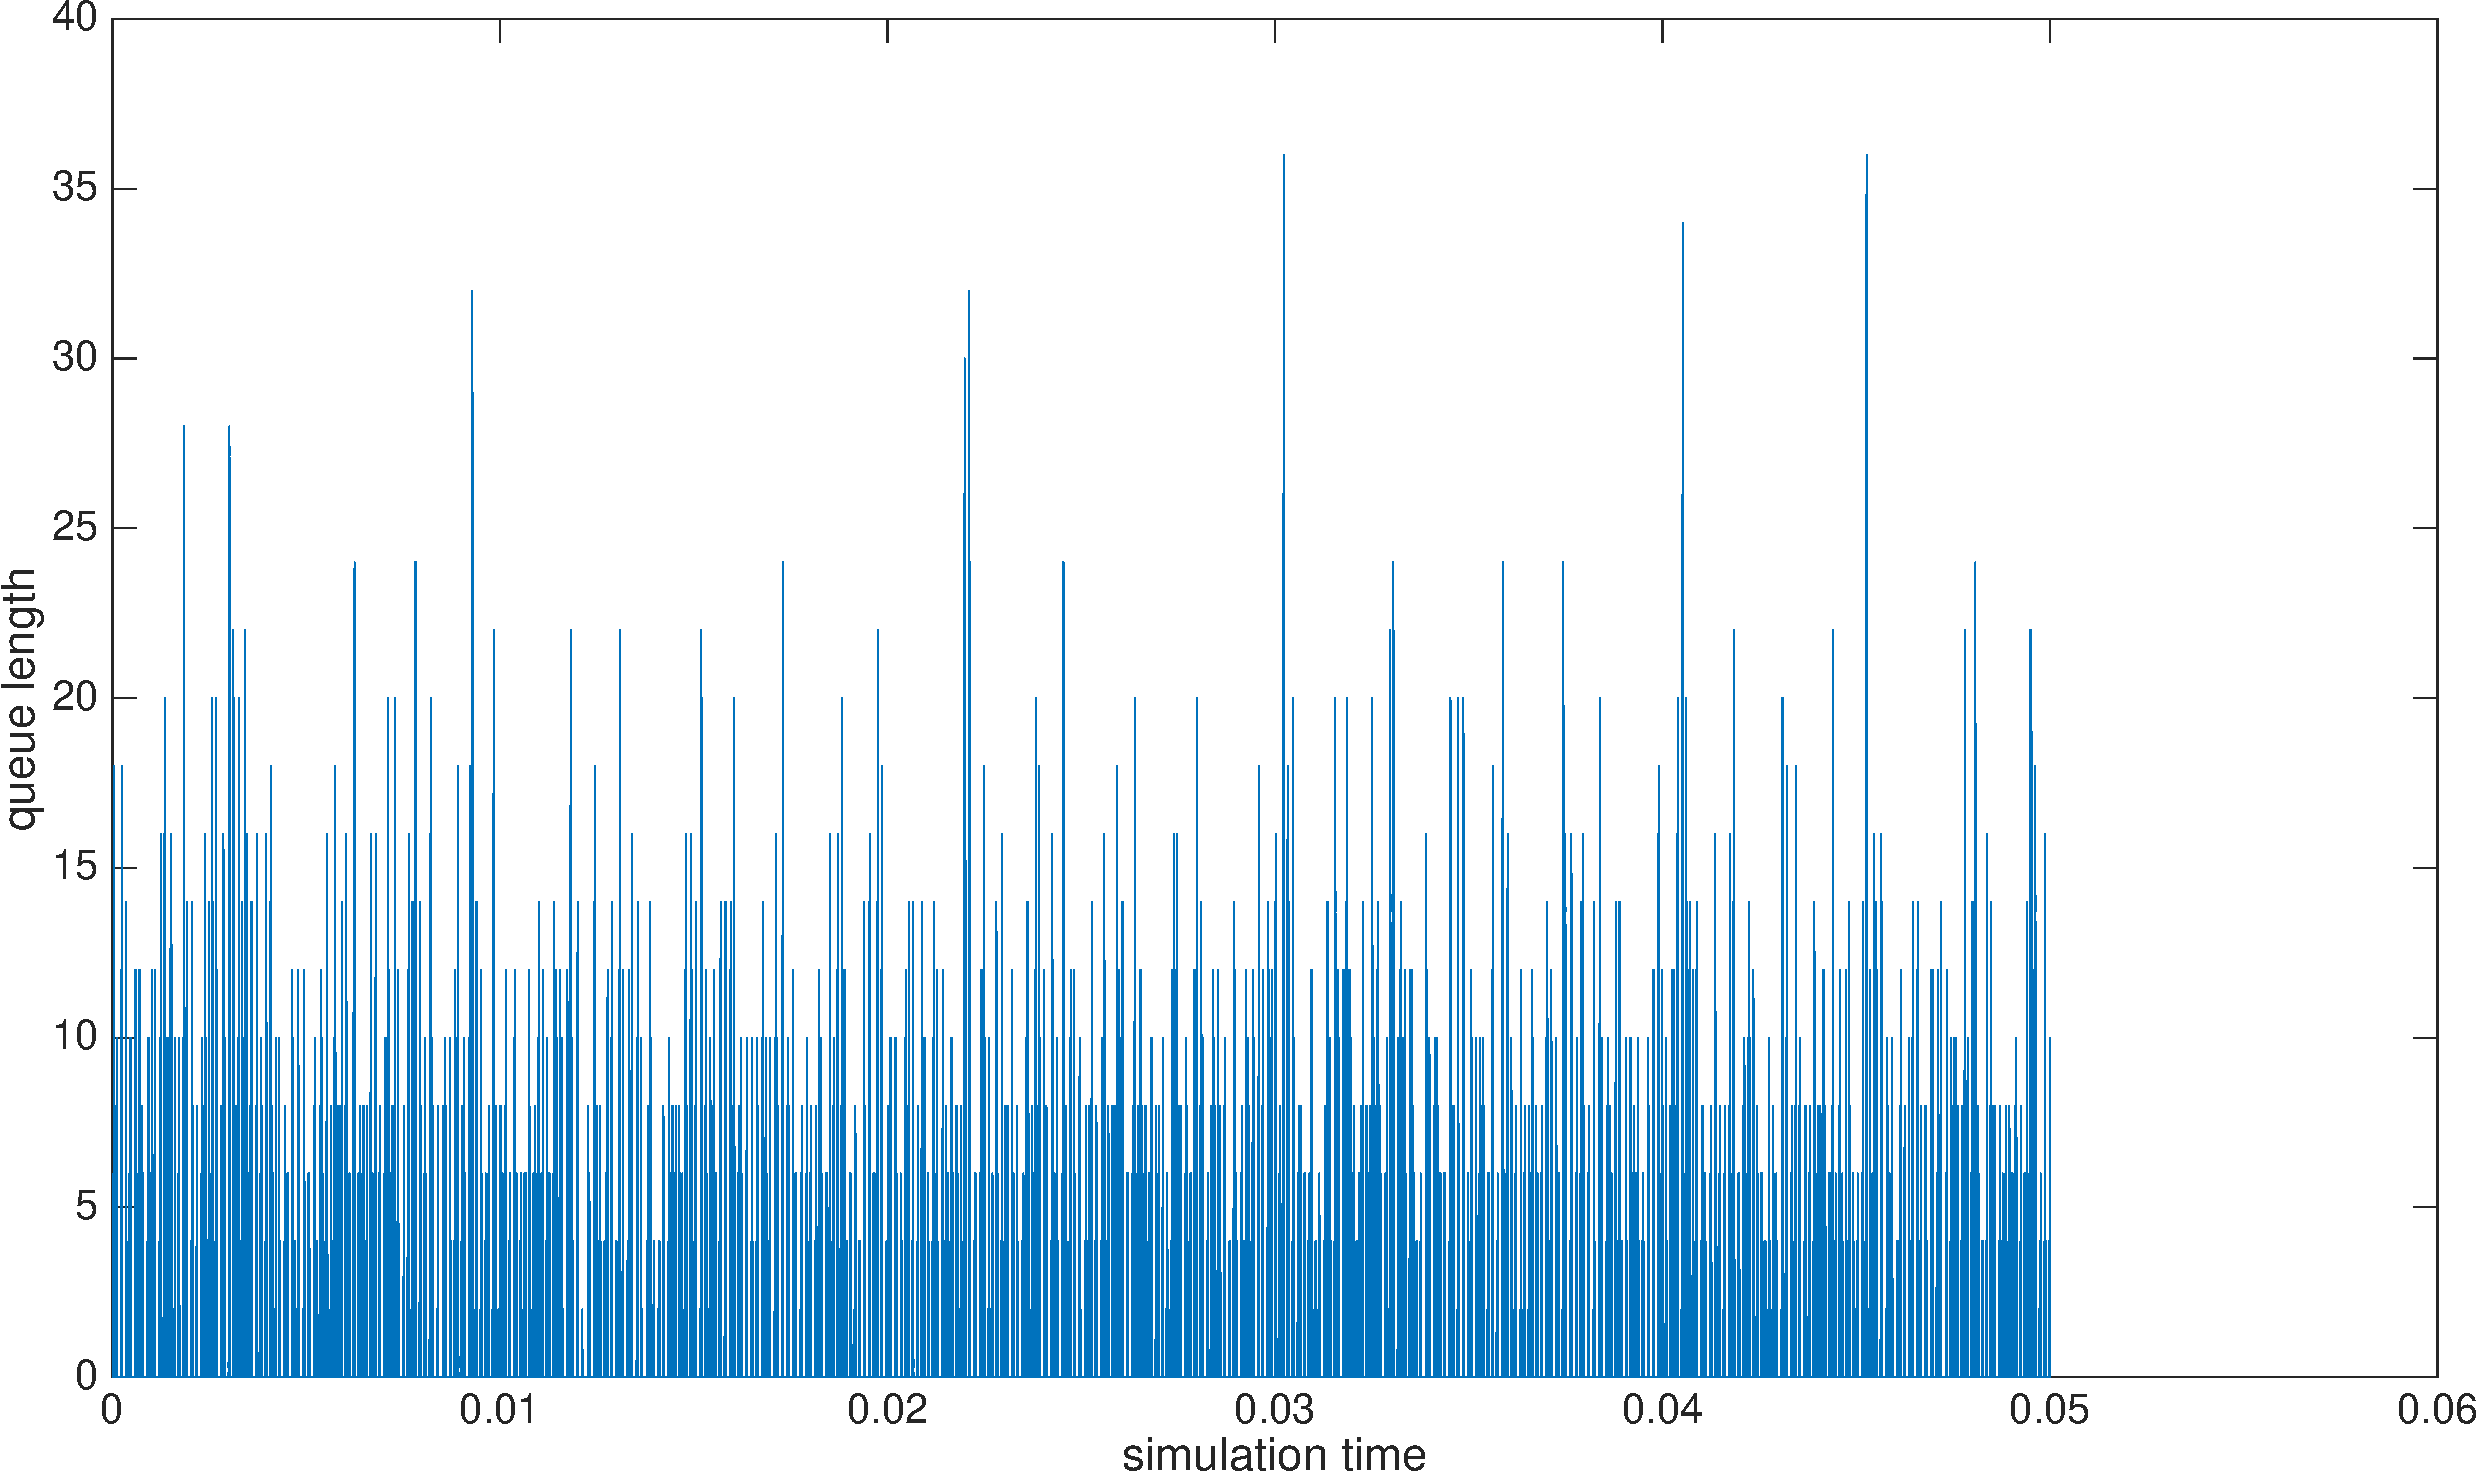
\includegraphics[width=\textwidth]{images/experiment/app2-queue2.pdf}
    \caption{Application 2: The number of tasks in the SSO/core queue, from the second resource usage queue.}
    \label{fig:app2-queue2}
  \end{center}
\end{figure}

\begin{figure}[]
  \begin{center}
    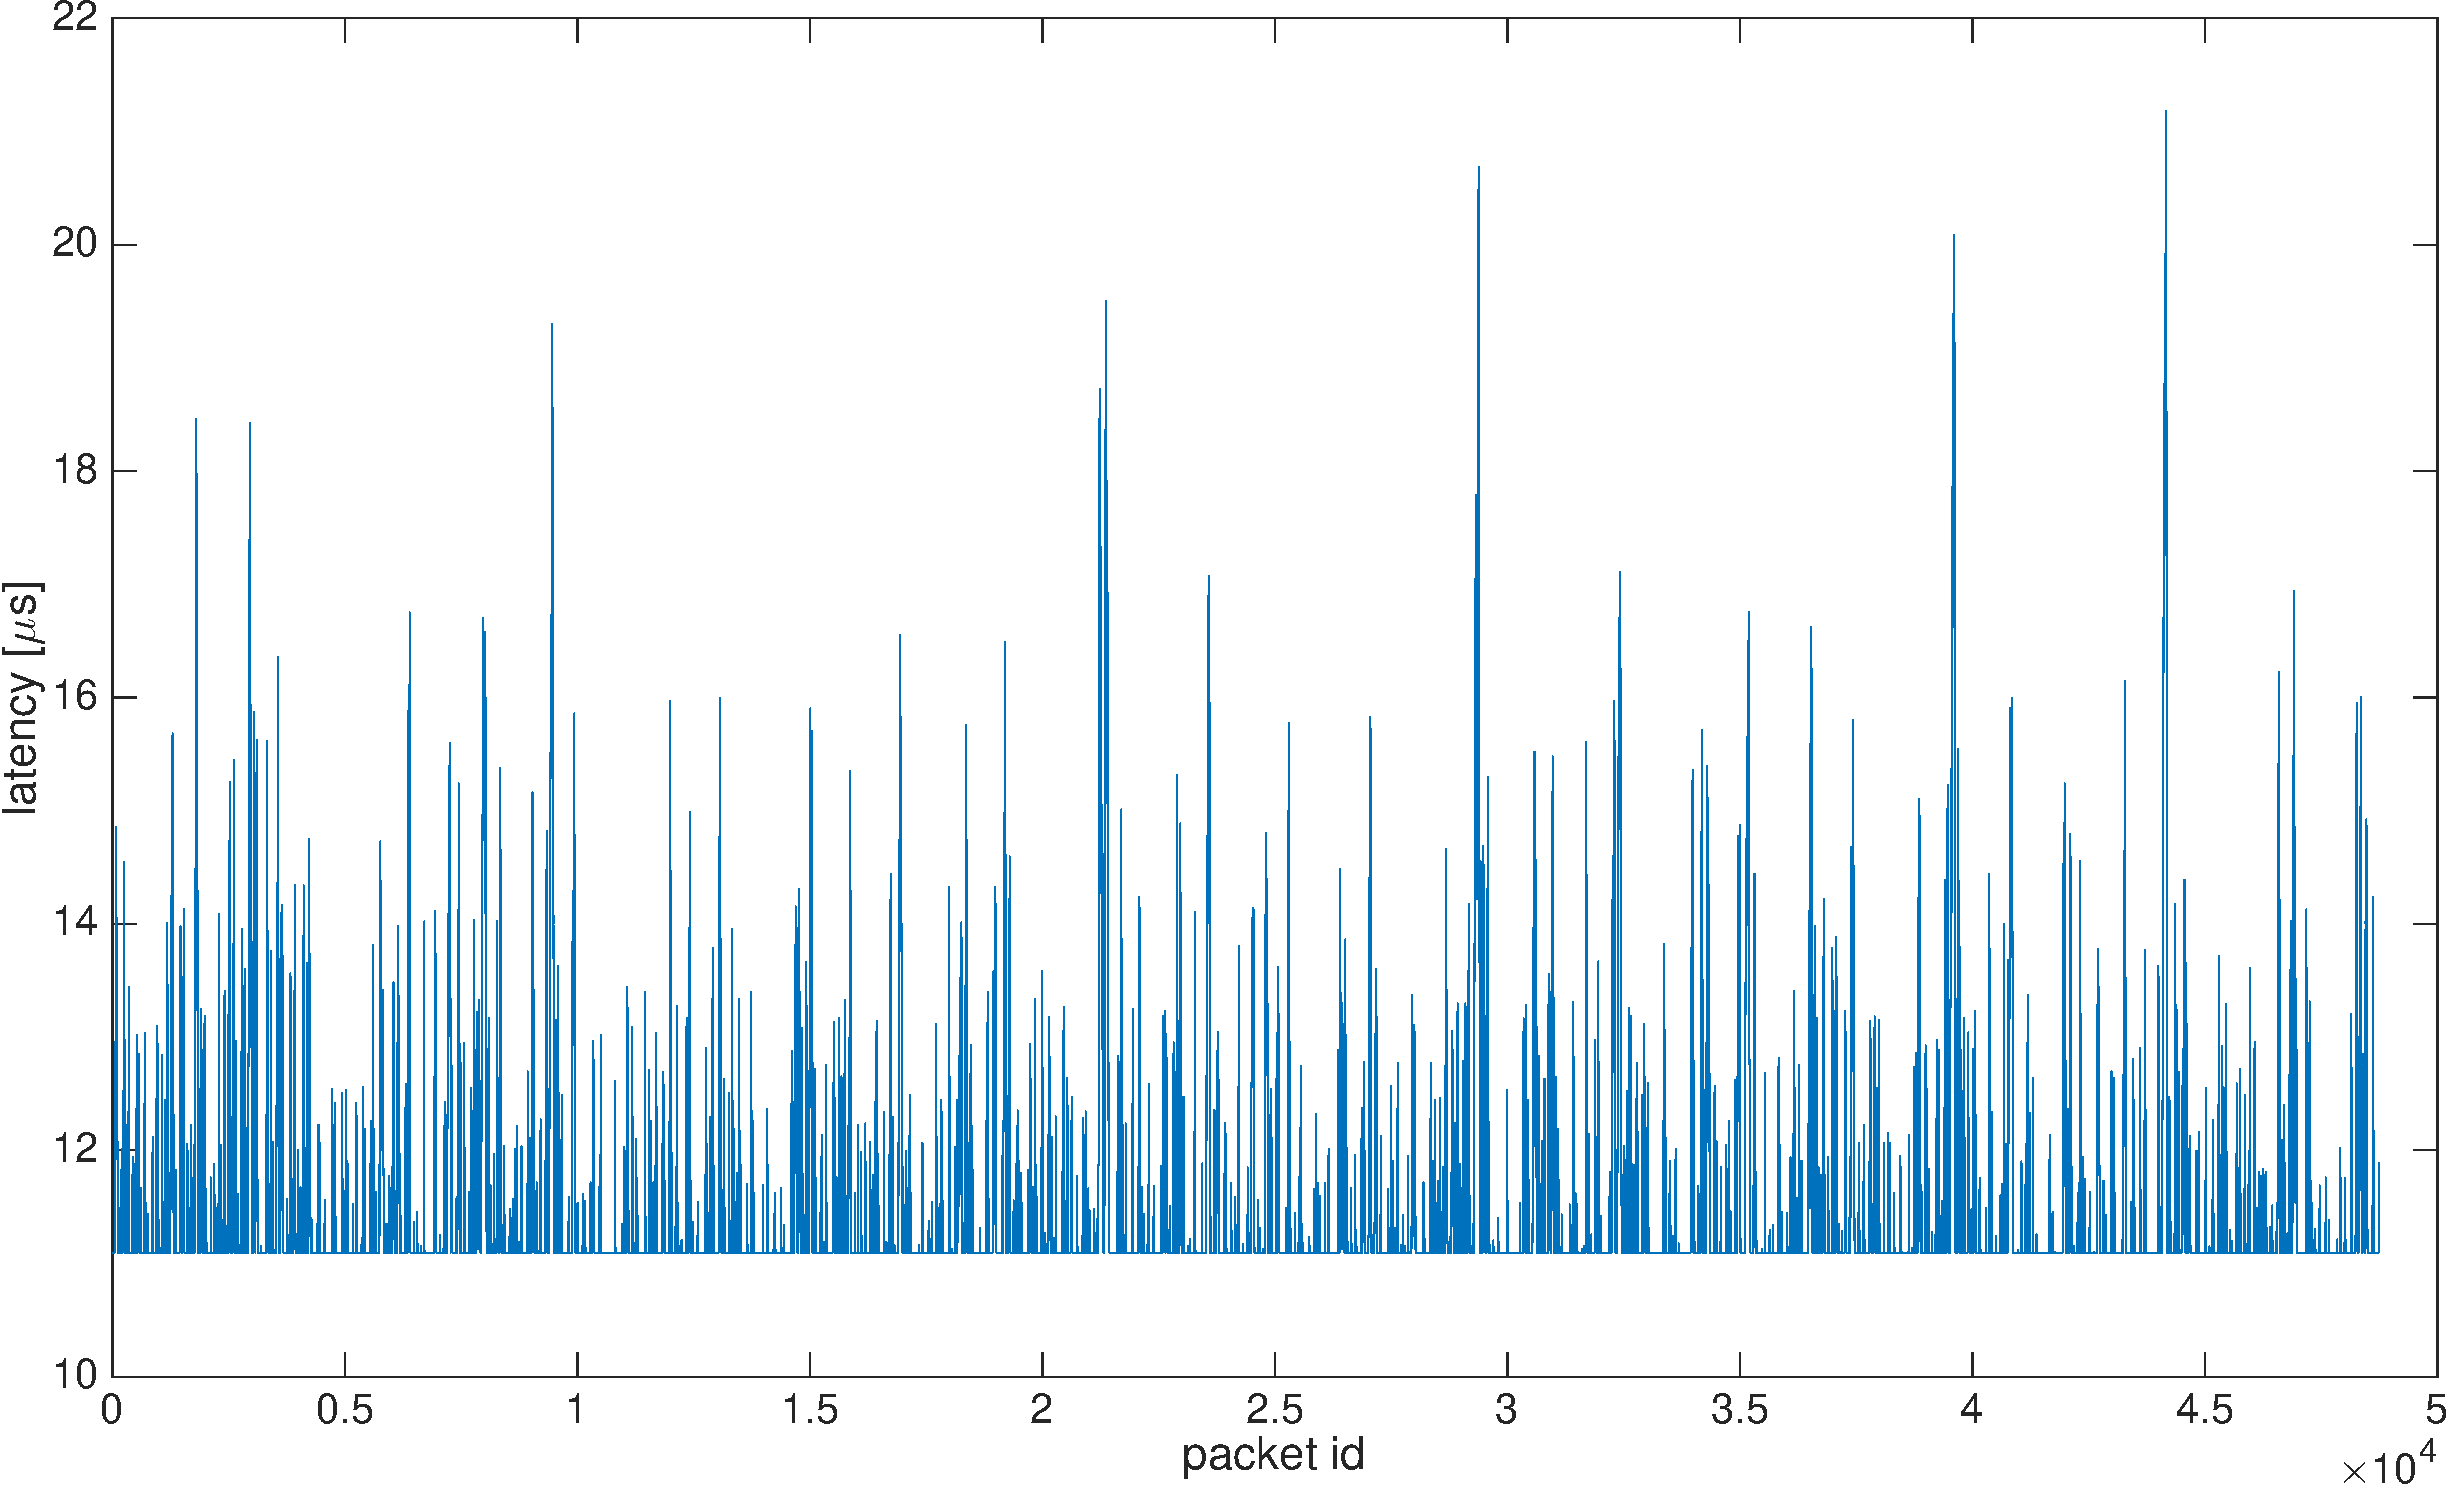
\includegraphics[width=\textwidth]{images/experiment/app2-latency.pdf}
    \caption{Application 2: Latency of the packets through the system.}
    \label{fig:app2-latency}
  \end{center}
\end{figure}

As the figures show, the second application removes the bottleneck from the system. The latencies stay within 22$\mu$s, and the limiting queue length is always below 40, over the simulation period.

\section{Discoveries}

The experiment presents an example usage of the PSE's plugin code mechanism and simulation of network processing unit. The simulation results are encouraging. First, they show that PSE can be used for performance analysis of more complex hardware accelerated systems. This brings advantages especially in the early design space exploration, when there are no real life system available, or when individual system parameters are explored.

The plugin code mechanism extends to any resource network based simulation task, providing flexibility, and allowing even more complex systems to be modeled.

%%% Local Variables:
%%% mode: latex
%%% TeX-master: "thesis-hartikainen"
%%% End:


\chapter{Discussion}
\label{chapter:discussion}

\section{Challenges}

\section{Discoveries}

\section{Related Work}

\section{Future Work}


%%% Local Variables:
%%% mode: latex
%%% TeX-master: "thesis-hartikainen"
%%% End:


\chapter{Conclusions}
\label{chapter:conclusions}

%%% Local Variables:
%%% mode: latex
%%% TeX-master: "thesis-hartikainen"
%%% End:



% Load the bibliographic references
% ------------------------------------------------------------------
% You can use several .bib files:
% \bibliography{thesis_sources,ietf_sources}
% \bibliography{sources}
\nocite{*}
\todo[inline]{remove nocite}
\printbibliography
% Appendices go here
% ------------------------------------------------------------------
% If you do not have appendices, comment out the following lines
% \appendix
% \chapter{First appendix}
\label{chapter:first-appendix}
\lstinputlisting[caption=RNS\_use\_device,
                 label=lst:RNS-use-device]{listings/RNS_use_device.c}

RNS\_use\_device in~\ref{lst:RNS-use-device} reserves the resource, delays the process (i.e. the task) and releases the resource for other processes.

\lstinputlisting[caption=RNS\_demand\_device,
                 label=lst:RNS-demand-device]{listings/RNS_demand_device.c}

RNS\_demand\_device routine in~\ref{lst:RNS-demand-device} is a simple wrapper routine, that converts the demanded service amount (service\_amount) into corresponding service time, based on the device entity speed (d-$\textgreater$speed). It then calls the RNS\_use\_device routine with the resulting service time.

\lstinputlisting[caption=RNS\_reserve\_resource,
                 label=lst:RNS-reserve-resource]{listings/RNS_reserve_resource.c}

\ref{lst:RNS-reserve-resource} summarizes the RNS\_reserve\_resource routine. RNS\_reserve\_resource calls the reserve function bound to the resource entity as explained in section \ref{TODO}. The reserve function assigns the task either in the resource's processing queue or waiting queue.

If the reserve function assigns the task to the waiting queue, the thread yields the execution to the scheduler.

\lstinputlisting[caption=RNS\_delay\_process,
                 label=lst:RNS-delay-process]{listings/RNS_delay_process.c}
\lstinputlisting[caption=RNS\_release\_resource,
                 label=lst:RNS-release-resource]{listings/RNS_release_resource.c}

%%% Local Variables:
%%% mode: latex
%%% TeX-master: "thesis-hartikainen.tex"
%%% End:


% End of document!
% ------------------------------------------------------------------
% The LastPage package automatically places a label on the last page.
% That works better than placing a label here manually, because the
% label might not go to the actual last page, if LaTeX needs to place
% floats (that is, figures, tables, and such) to the end of the
% document.
\end{document}

%%% Local Variables:
%%% mode: latex
%%% TeX-master: t
%%% End:
